%------------------------------------------------
\chapter{\textbf{Resultados Experimentais obtidos na solução do labirinto}}\label{Resultados}
%---------------------------------------------------------


Este capítulo apresenta os resultados observados e as análises realizadas a partir dos testes nas partes implementadas. A divisão das seções é a mesma anteriormente apresentada para a apresentação dos resultados individualmente. Finalmente, é realizada uma análise geral do sistema como um todo.

\section{\textit{Hardware}}
% Descrever alguns testes com o robô
Os primeiros testes foram realizados com o robô, a fim de determinar algumas informações importantes, tais como número de pulsos por revolução gerados, verificação das relações de tensão por distância dos sensores de distância e comunicação via \textit{bluetooth}. Estas informações são usadas nos algoritmos implementados.

Para validação do número de pulsos gerados por volta completa do eixo do motor, um programa básico foi utilizado. O módulo QEI do microcontrolador analisa os dois canais do \textit{encoder} e incrementa um contador.

\subsection{Sensores de distância infravermelhos}
Testes foram feitos, com os sensores IR, e foi constatado que o valor de \emph{tensão} aumenta à medida que o robô se aproxima do obstáculo, conforme pode ser observado na Figura \ref{fig:IR_frontal}. As medidas de distância foram realizadas do eixo das rodas até o obstáculo à frente.

\begin{figure}[!htb]
	\caption{\label{fig:IR_frontal}Parede à frente}
	\begin{center}
		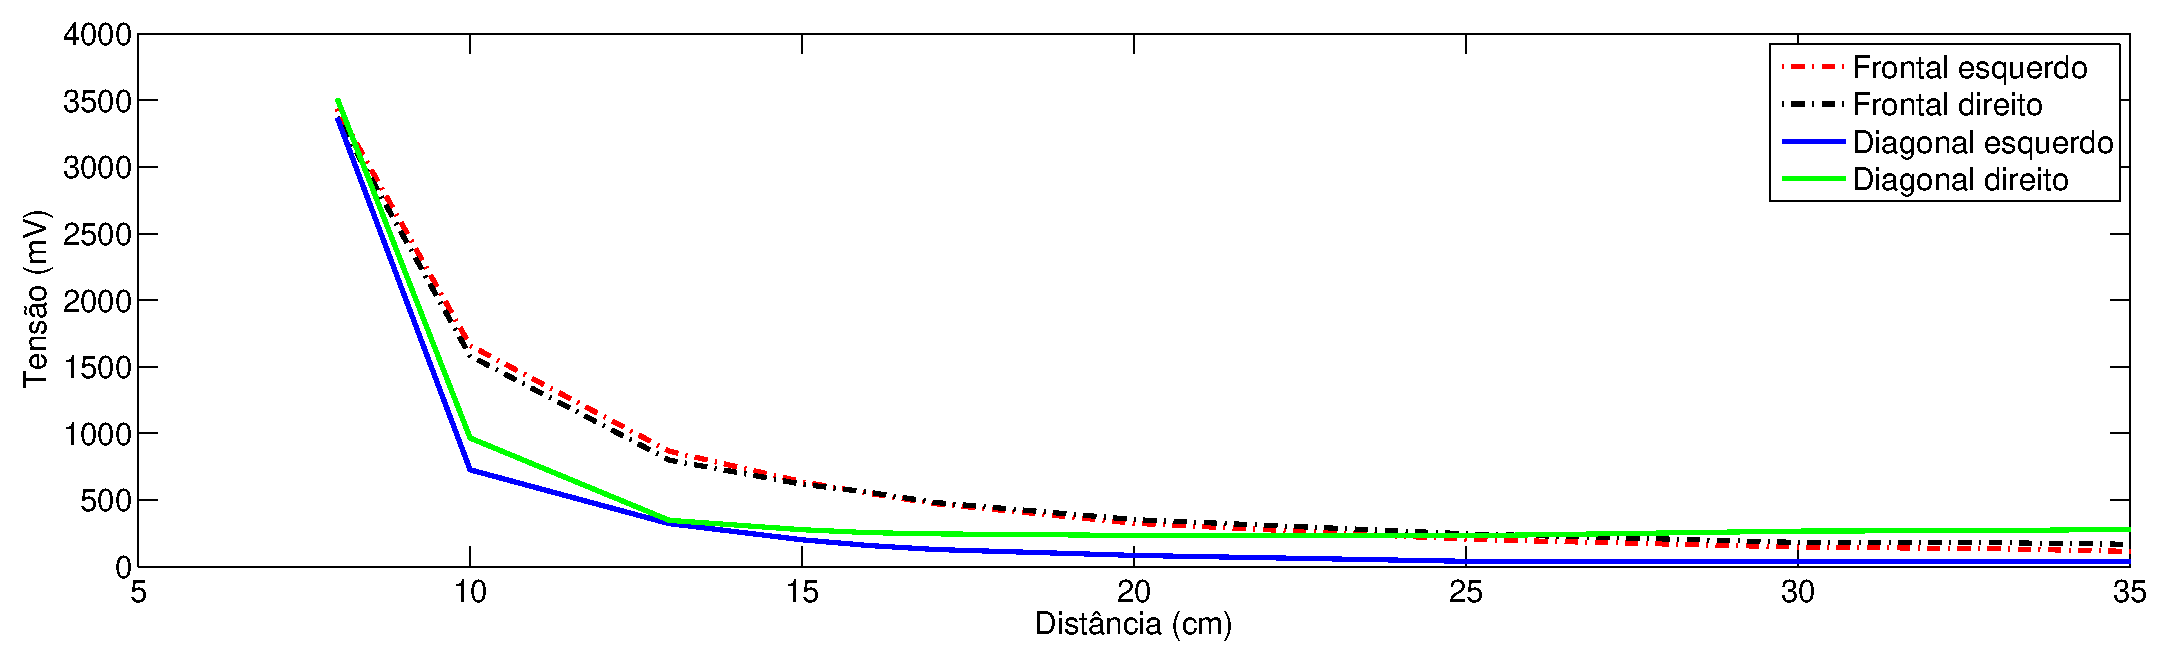
\includegraphics[width=1\linewidth]{sensores.eps}
	\end{center}
	\legend{Fonte: autor (2017)}
\end{figure}

As medidas dos sensores frontais se diferenciaram dos sensores diagonais, porque os obstáculos se localizaram de frente com o robô.

Com os gráficos, pode-se determinar limiares de detecção de parede, que, através deles, são definidos os três bits da função de leitura dos sensores. A Figura \ref{fig:sensor_bin} mostra os três bits para todas as possibilidades de obstáculos à frente.

\begin{figure}[!htb]
	\caption{\label{fig:sensor_bin}Retorno da função \texttt{getSensoresParede()} com obstáculos à frente}
	\begin{center}
		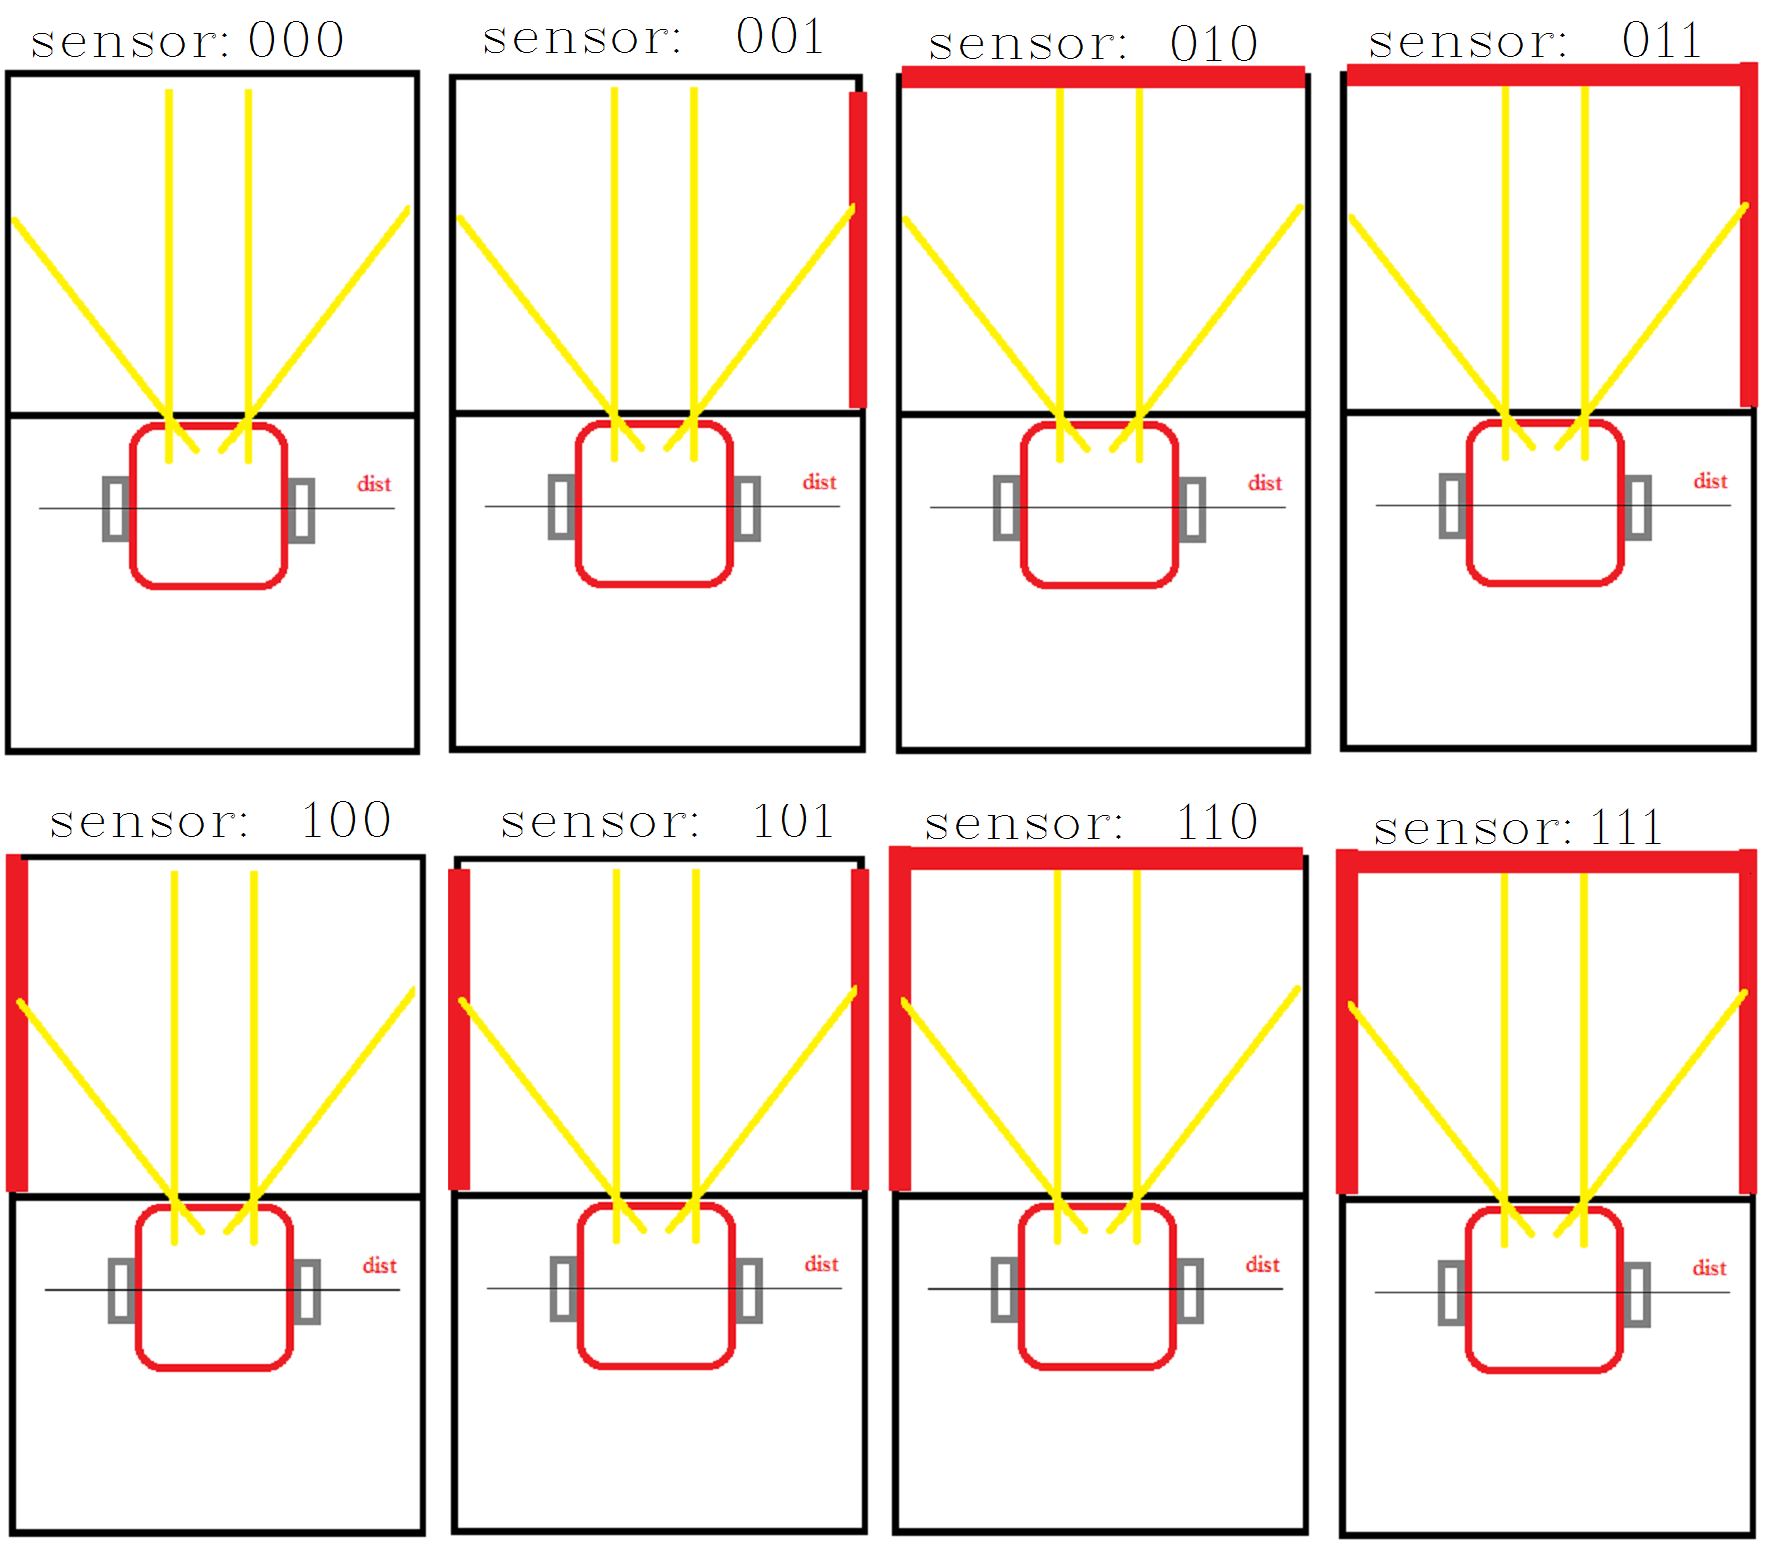
\includegraphics[width=.6\linewidth]{sensores.png}
	\end{center}
	\legend{Fonte: autor (2017)}
\end{figure}

Os limiares para detecção de paredes foram determinados da seguinte forma, considerando sempre a pior posição para a medida das distâncias: 

\begin{enumerate}[leftmargin=2cm,label=\alph*)]
\item o robô é posicionado sempre na célula anterior, para detectar as paredes da célula seguinte a tempo do algoritmo de resolução indicar a nova orienteção e sentido;
\item para detecção da parede à frente, a distância do eixo das rodas até o vértice da próxima célula é de 6 cm, consequentemente, a 24 cm do obstáculo; 
\item para detecção da parede lateral, o robô era posicionado no canto oposto;
\item realizou-se a leitura dos sensores para cada condição mostrada na Figura \ref{fig:sensor_bin};
\item a medida mínima realizada para cada sensor era considerada para limiar de detecção das paredes.
\end{enumerate}

A Tabela \ref{tab:limiares_sensores} mostra os limiares obtidos experimentalmente.

\begin{table}[!htb]
	\centering
	\caption{\label{tab:limiares_sensores}Valor mínimo de tensão para detecção das paredes}
	\begin{tabular}{c|c}
	 \textbf{Sensor} & \textbf{Tensão} ($mV$) \\ 
	 \hline 
	 \textbf{Frontal} & 220 \\ 
	 \hline 
	 \textbf{Diagonal esquerdo} & 600 \\ 
	 \hline 
	 \textbf{Diagonal direito} & 240 \\ 
	 \end{tabular}  
	
	\legend{Fonte: autor (2017)}
\end{table}

%\begin{figure}[!htb]
%	\caption{\label{fig:IR_esq}Parede à esquerda}
%	\begin{center}
%		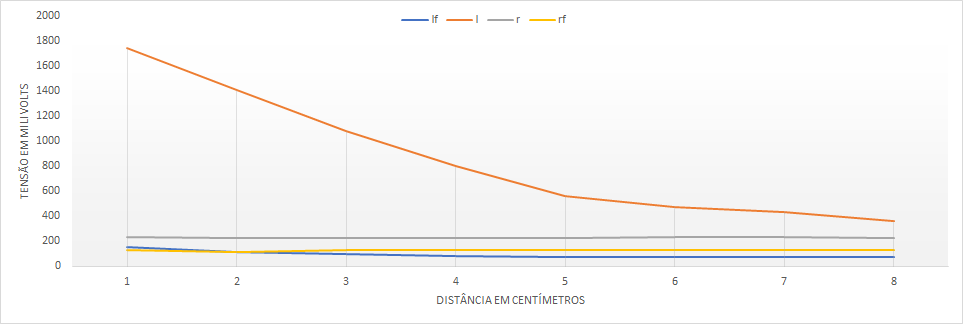
\includegraphics[width=.9\linewidth]{parede_a_esq.png}
%	\end{center}
%	\legend{Fonte: autor (2017)}
%\end{figure}
%
%\begin{figure}[!htb]
%	\caption{\label{fig:IR_dir}Parede à direita}
%	\begin{center}
%		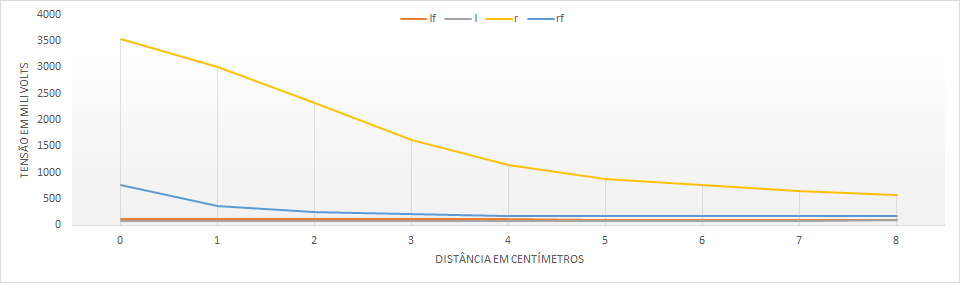
\includegraphics[width=.9\linewidth]{parede_a_dir.png}
%	\end{center}
%	\legend{Fonte: autor (2017)}
%\end{figure}

\subsection{\textit{Encoders}}
	Um teste foi feito para determinar a quantidade de pulsos, com o objetivo de conhecer o valor certo de número de pulsos por volta. Em cada roda, uma marcação de referência foi realizada. Um programa simples para este teste foi gravado no micromouse e a cada segundo era retornado o valor do registrador. Em cada roda, uma volta completa foi girada com a mão. Os \textit{encoders} geram 358 pulsos por volta, ao invés de 360 pulsos.



\section{Algoritmo}

O resultado da construção do algoritmo no \textit{FALCON C++ IDE} pode ser observado visualmente, através dos símbolos, no próprio programa compilado. Mais à frente, é mostrado o algoritmo teste real, que será feito em conjunto com o controle em malha fechada do Micromouse.

\subsection{Modelando um labirinto}
Os resultados observados do algoritmo desenvolvido no \textit{FALCON C++ IDE} dependem da modelagem do labirinto. Para tanto, foi criada mais uma variável dentro da estrutura de dados da célula, que, por sua vez, pode ser acessada através de \verb+celula[x][y].parede[z]+. Desta forma, os bits das paredes da célula à frente podem ser utilizados pelo algoritmo, quando solicitado, para emular os sensores de distância do Micromouse.

No algoritmo, uma função de inicialização realiza a leitura de dois arquivos de extensão $.txt$ (arquivos que contém os bits das paredes horizontal e vertical) e atualiza na estrutura de dados todas as paredes do labirinto modelado. Desta forma, pode-se simular qualquer labirinto e certificar-se do correto funcionamento do algoritmo criado, até mesmo comparar os resultados com o simulador \emph{Micro Mouse Maze Editor and Simulator}.

%\begin{figure}[!htb]
%	\caption[Modelagem de um labirinto para simulação]{\label{fig:ModelagemLab2}Modelagem de um labirinto}
%	\begin{center}
%		\subfloat[Design do labirinto \emph{Seoul 01}]{\includegraphics[width=0.4\linewidth]{modelagem_labirinto.png}}
%		\hspace*{0.1\linewidth}
%		\subfloat[Resultado da conversão do labirinto]{\includegraphics[width=0.4\linewidth]{modelagem_labirinto2.png}}
%	\end{center}
%	\centering
%	\small Fonte: autor (2017)
%\end{figure}


Através do \textit{EXCEL}, foi criada uma plataforma \textit{conversora} de labirinto. Visualmente pode-se configurar as paredes, e o mesmo é encarregado de gerar informações binárias necessárias para executar o algoritmo criado no \textit{FALCON C++ IDE}. As colunas e linhas são comprimidas e preenchidas com cores para dar forma às paredes, conforme pode ser observado com detalhes na Figura \ref{fig:Modelagem}.

\begin{figure}[!htb]
	\caption{\label{fig:Modelagem}\textit{EXCEL} como ferramenta para modelagem de labirinto}
	\begin{center}
		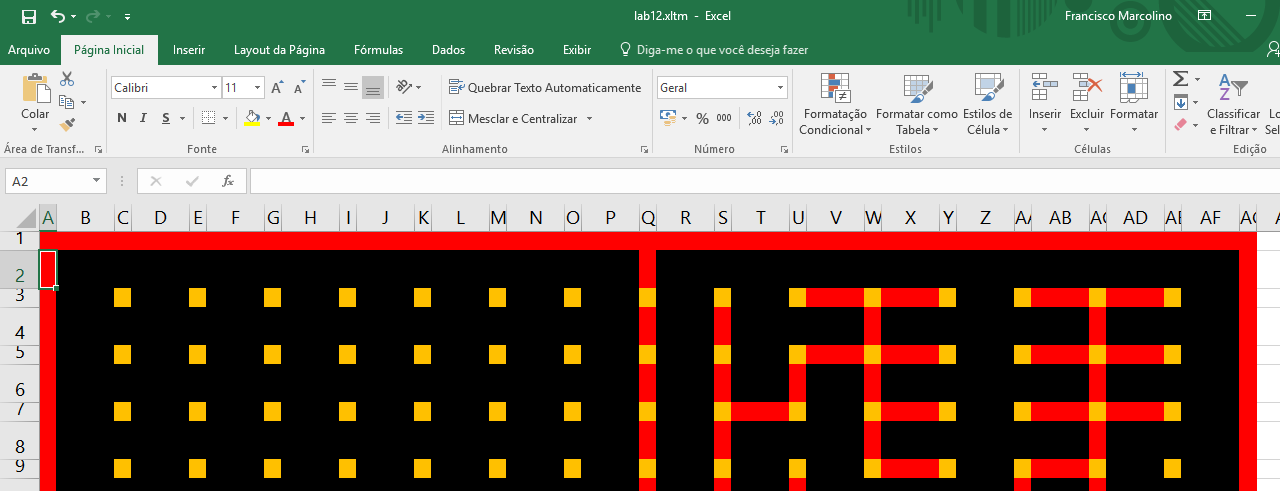
\includegraphics[width=1\linewidth]{excel.PNG}
	\end{center}
	\legend{Fonte: autor (2017)}
\end{figure}

Os \textit{bits} são formados através das fórmulas, que são inseridas nas células. As fórmulas são equações que podem executar cálculos, retornar informações, manipular o conteúdo de outras células, testar condições e mais. Uma fórmula sempre começa com um sinal de igual (=). Uma função macro do \textit{EXCEL} foi utilizada para detectar cores de preenchimento, e ela retorna o número da cor. Desta forma, se a cor da célula é vermelha (número 255), então significa que existe uma parede e o \textit{bit} 1 será selecionado pela função lógica condicional "SE", do \textit{EXCEL}. Caso contrário, o valor gerado é 0. Logo a seguir é mostrada a fórmula para gerar o \textit{bit} na célula B1, por exemplo:

\begin{verbatim}
=SE(gfCelColorName(B1)="255";"1";"0")
\end{verbatim}

Na Figura \ref{fig:Modelagem}, o valor retornado pela fórmula é 1, porque a célula B1 do \textit{EXCEL} está preenchida com a cor vermelha. Desta forma, as matrizes de \textit{bits} das paredes horizontais e verticais são geradas.

\begin{figure}[!htb]
	\caption{\label{fig:ModelagemLabirinto}Modelagem do labirinto \textit{Seoul} para simulação}
	\begin{center}
		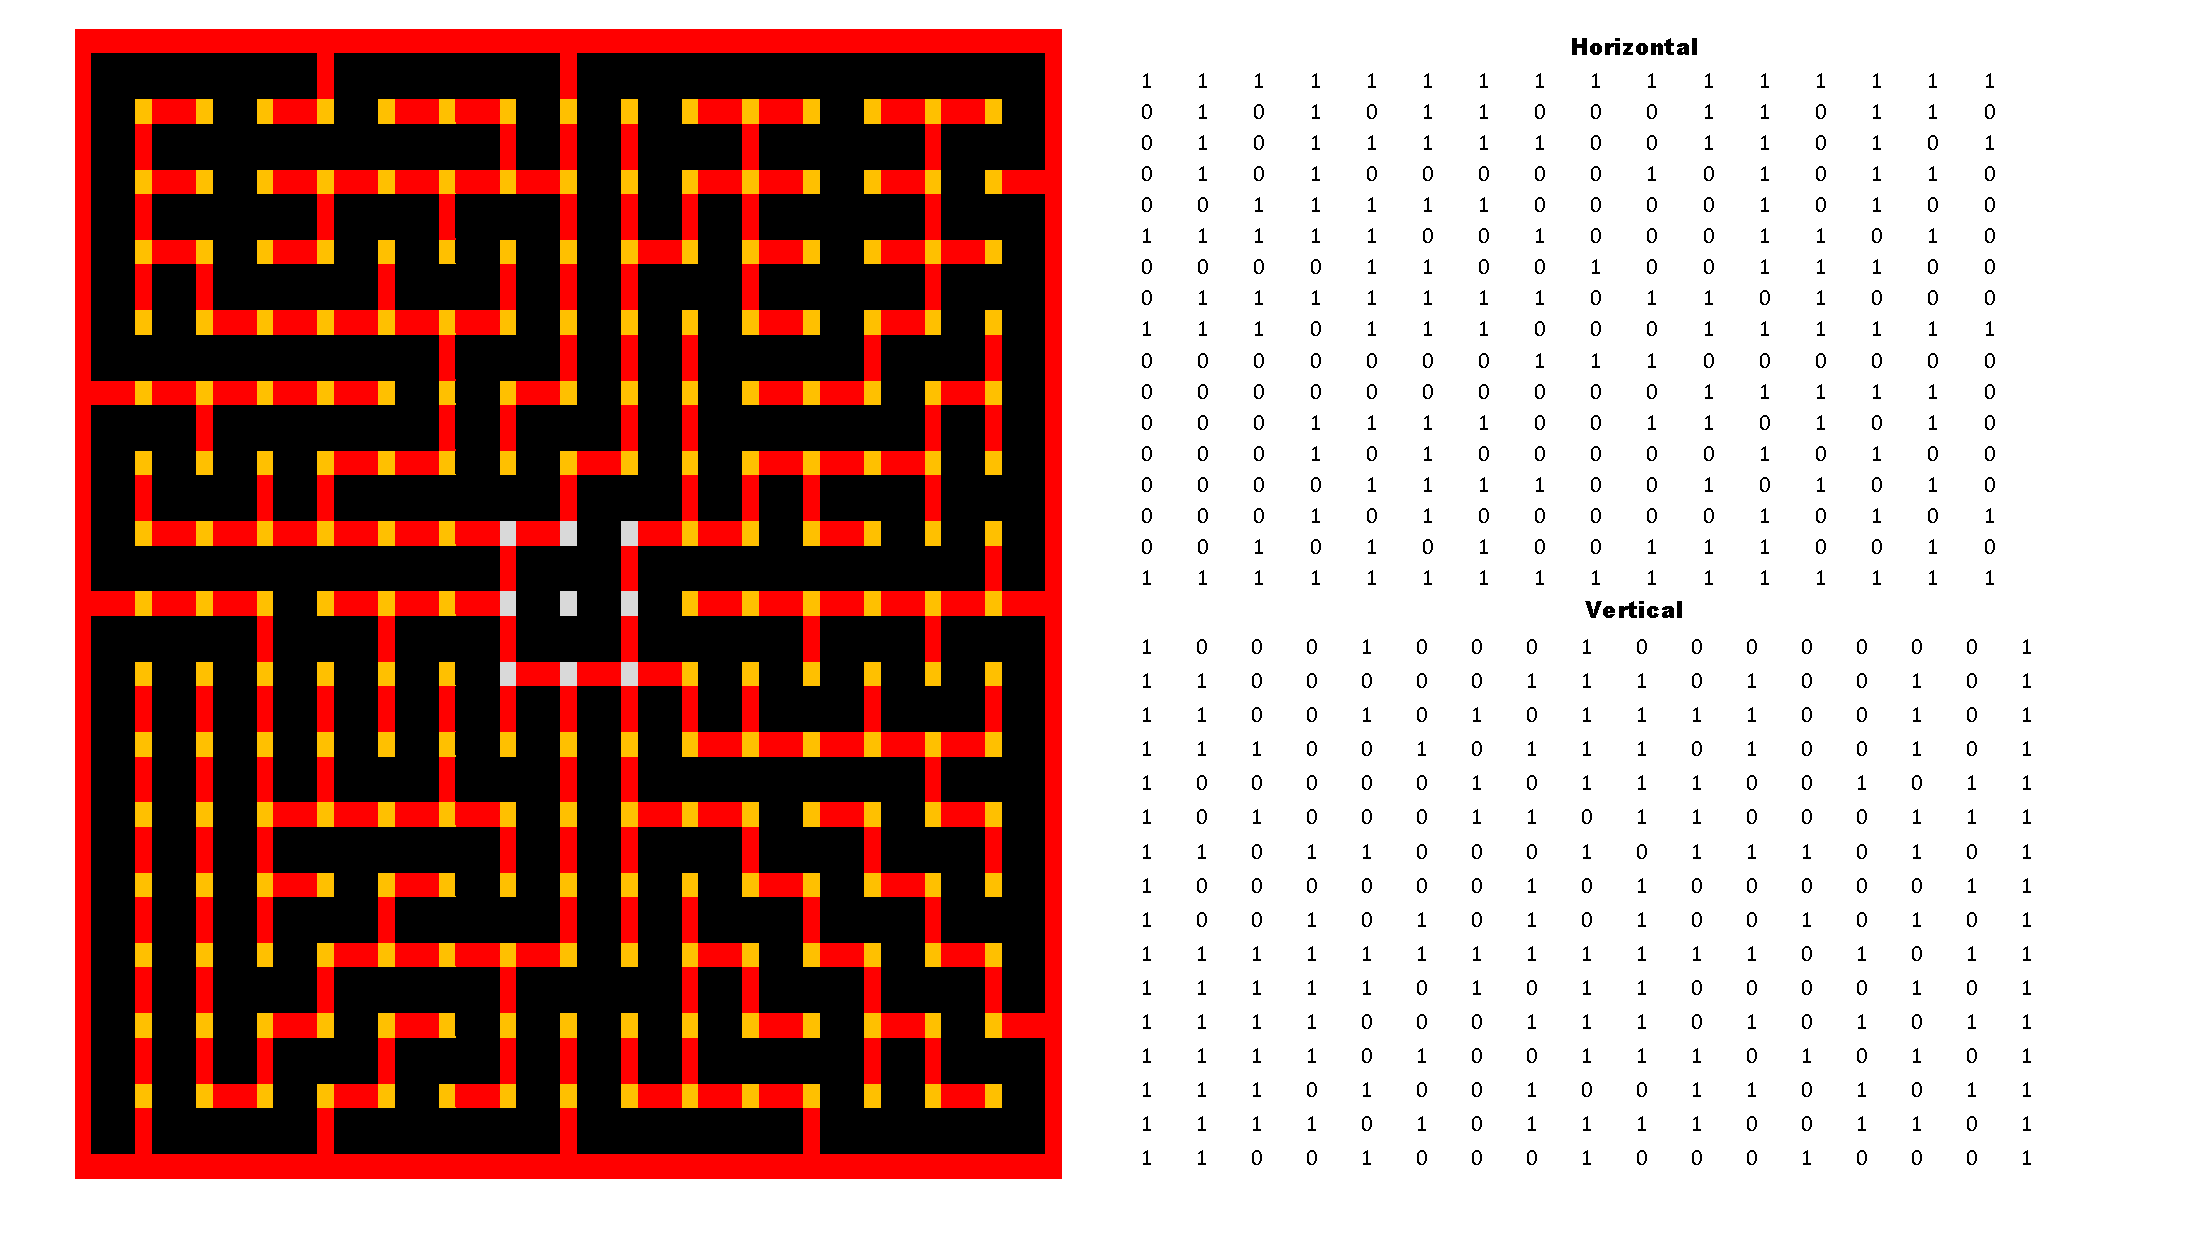
\includegraphics[width=1\linewidth]{SEOL01.pdf}
	\end{center}
	\legend{Fonte: autor (2017)}
\end{figure}


A Figura \ref{fig:ModelagemLabirinto} mostra a modelagem de um labirinto \emph{Seoul 01} no \textit{EXCEL}, design de labirinto que exige esforço do algoritmo, ideal para testes. Logo ao lado da figura contém as matrizes binárias prontas para exportar para arquivos $.txt$.

\subsection{Simulando o algoritmo no labirinto}

Para validação do algoritmo construído, foi utilizado o desenho do labirinto \emph{Seoul 01}, Figura \ref{fig:ModelagemLabirinto}, disponibilizado para testes no simulador \emph{Micro Mouse Maze Editor and Simulator}. Segundo as estatísticas para o labirinto, cerca de 694 células devem ser atravessadas para completar a melhor corrida, e pela dificuldade, ele foi adotado para simulação.

Após modelar o labirinto escolhido, os arquivos $.txt$ são atualizados através das matrizes de bits gerados pelo \textit{EXCEL}. E no programa \textit{FALCON C++ IDE}, o algoritmo é compilado e executado, de forma que apareça na janela de \emph{Prompt de Comandos} do \emph{Windows} os símbolos para modelagem do labirinto. 

A cada estado, o programa imprime uma mensagem com o nome do estado em que o algoritmo se encontra, como pode ser visto na Figura \ref{fig:simulacao1}. 
No estado \texttt{IMPRIMIR MAZE}, o algoritmo imprime de fato todo o labirinto visto pelo robô, ou seja, as paredes descobertas por ele, incluindo as marcações nas células visitadas e também o símbolo de direção e sentido na célula a qual o robô se encontra. Quando o robô chega no estado \verb+ESPERAR_CELULA+, o programa espera o pressionar do \textit{ENTER} para o algoritmo voltar para o estado \verb+MOVER_ROBO+ e prosseguir com o percurso de forma virtual. Desta forma, uma lista impressa é gerada e o percurso do robô pode ser acompanhado. Também é possível o acompanhamento da atualização das distâncias das células, quando é preciso, a cada passo dado.


\begin{figure}[!htb]
	\caption{\label{fig:simulacao1}Acompanhamento e simulação do algoritmo proposto}
	\begin{center}
		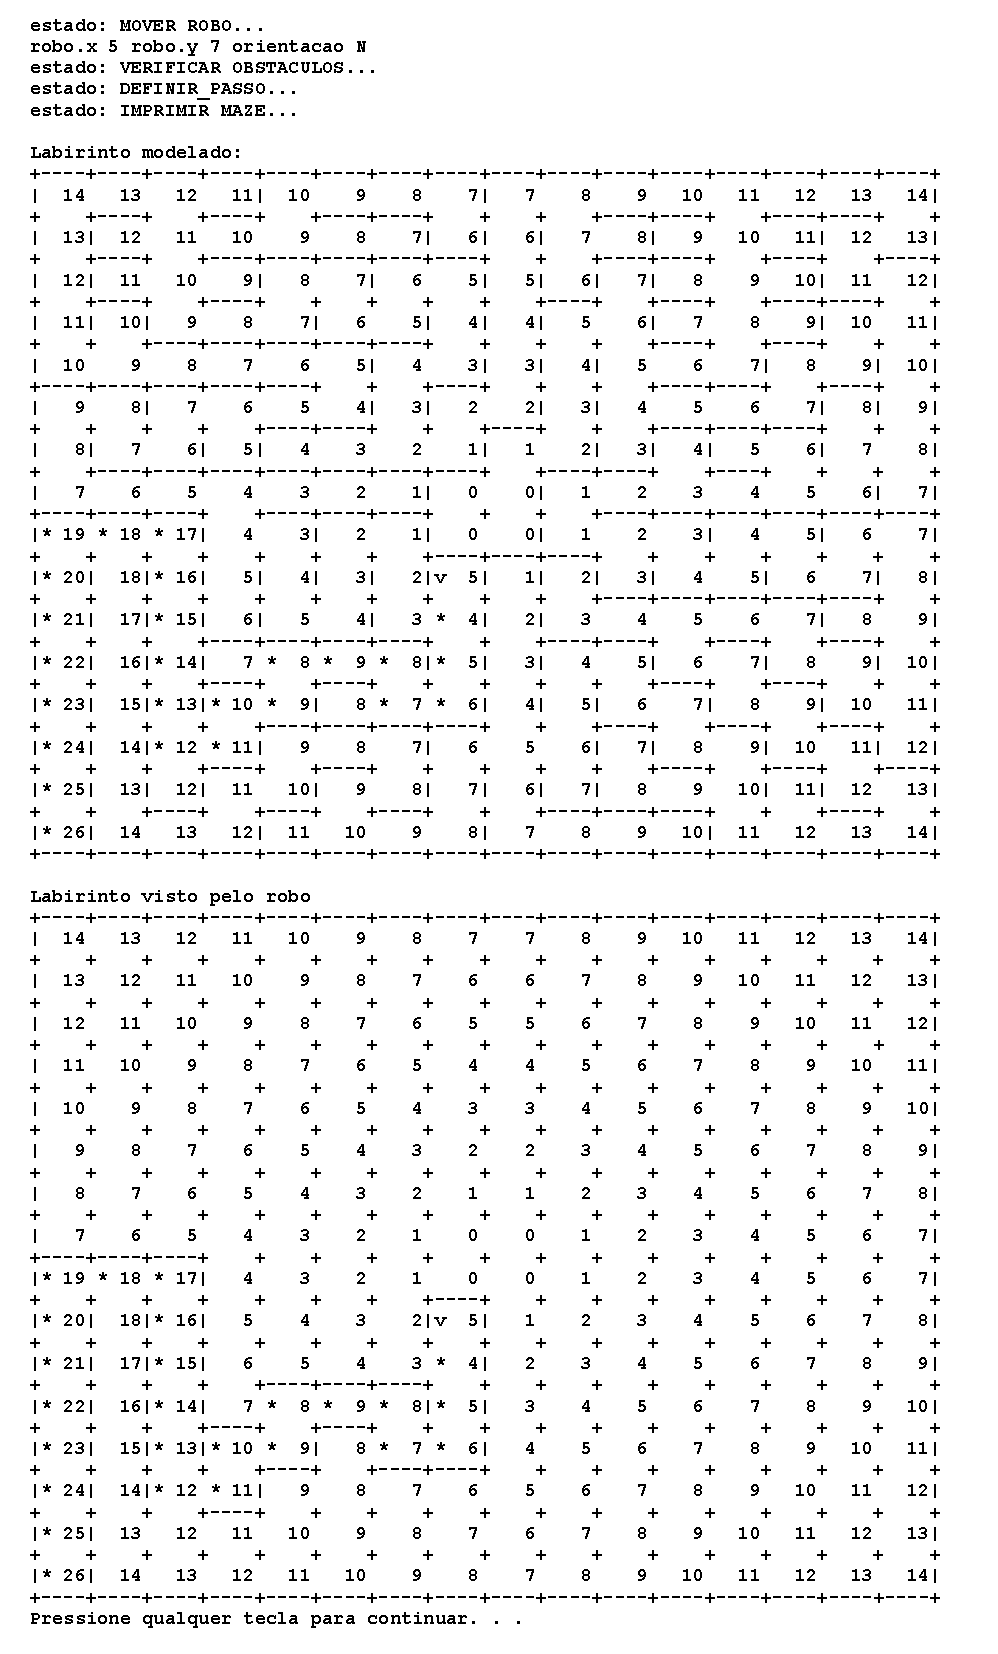
\includegraphics[width=0.6\linewidth]{simulacao1.pdf}
	\end{center}
	\centering
	\small Fonte: autor (2017)
\end{figure}


Para validação do algoritmo, foram realizadas comparações das distâncias das células a cada percurso virtual dos simuladores.


A Figura \ref{fig:ModelagemLab2} (a) mostra a distribuição das distâncias ao final de uma corrida, com detalhe na marcação das células visitadas com asterisco (em verde). Em comparação com o percurso do algoritmo do simulador \emph{Micro Mouse Maze Editor and Simulator} da Figura \ref{fig:ModelagemLab2} (b), são bastante idênticos ambos os percursos. Prioridade para escolha da orientação entre vizinhanças de mesmo número, nos algoritmos de tomada de decisão, causam estas pequenas diferenças entre os percursos. Porém, nas simulações, observou-se que o algoritmo proposto converge sempre para o mesmo caminho do algoritmo do simulador \emph{Micro Mouse Maze Editor and Simulator}, ao aumentar o número de corridas.


\begin{figure}[!htb]
	\caption[Percurso do robô no labirinto \emph{Seoul} - primeira corrida \emph{real}]{\label{fig:ModelagemLab2}Percurso do robô no labirinto Seoul - primeira corrida real}
	\begin{center}
		\subfloat[Algoritmo proposto]{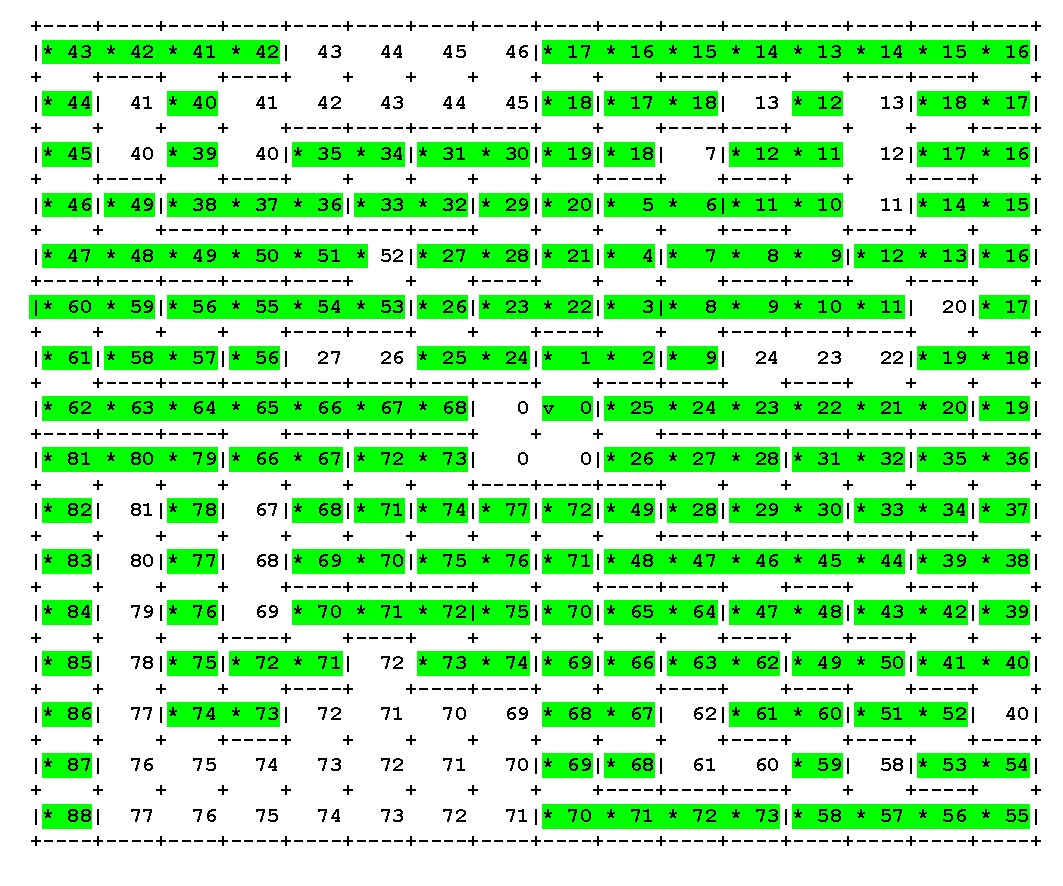
\includegraphics[width=0.45\linewidth]{seol01_1.pdf}}
		\hspace*{0.1\linewidth}
		\subfloat[Simulador Micromouse]{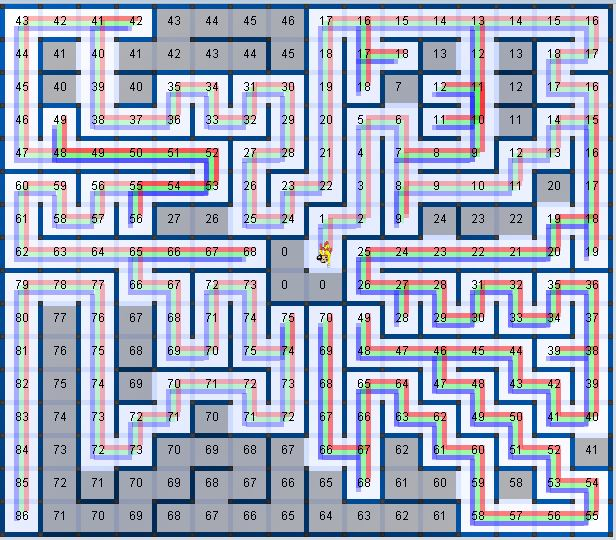
\includegraphics[width=0.4\linewidth]{seol01_2.JPG}}
	\end{center}
	\centering
	\small Fonte: autor (2017)
\end{figure}


%\begin{figure}[!htb]
%	\caption{\label{fig:seoul01_1}Percurso do robô no labirinto \emph{Seoul} com algoritmo criado na primeira corrida \emph{real}}
%	\begin{center}
%		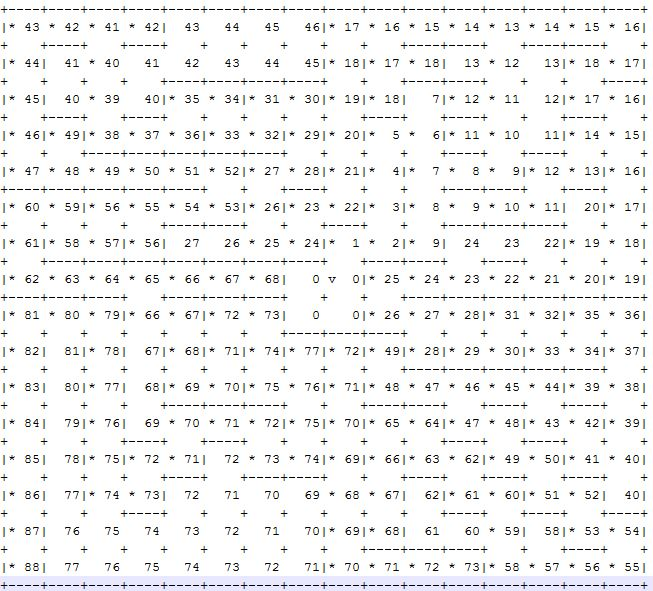
\includegraphics[width=1.0\linewidth]{seol01_1.JPG}
%	\end{center}
%	\centering
%	\small Fonte: do autor
%\end{figure}
%
%
%\begin{figure}[!htb]
%	\caption{\label{fig:seoul01_2}Percurso do robô no labirinto \emph{Seoul} com algoritmo do \emph{Micro Mouse Maze Editor and Simulator}}
%	\begin{center}
%		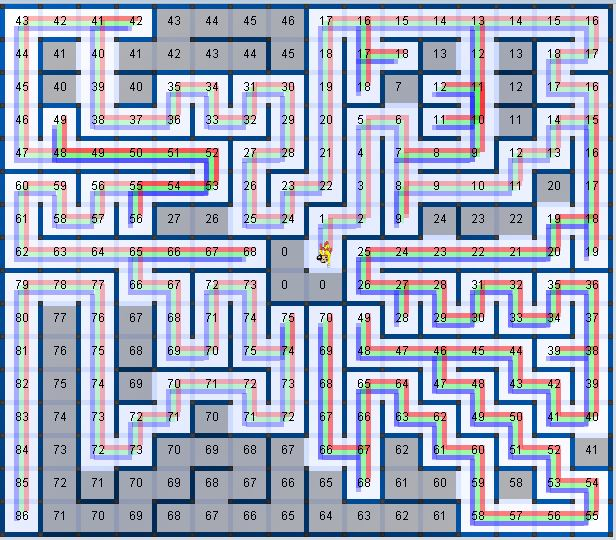
\includegraphics[width=1.0\linewidth]{seol01_2.JPG}
%	\end{center}
%	\centering
%	\small Fonte: do autor
%\end{figure}

No algoritmo proposto, a cada corrida (tanto da IDA como da VOLTA) as distâncias das células são reinicializadas, porém, as informações das paredes descobertas permanecem em RAM. Com esta estratégia, utilizando a mesma estrutura de memória, resulta em uma economia de 50\%\ de \emph{RAM} neste quesito.

Então, ao final de uma corrida, as distâncias das células são redefinidas e inicia-se a \emph{varredura virtual} do robô. A condição de parada é obtida quando o número de passos da corrida anterior se torna idêntico ao número de passos da última tentativa, em um processo de aproximação sucessiva. Assim, o robô poderá sair da célula central à celula de partida seguramente na menor distância possível para voltar em seguida. 

Para o labirinto em questão, foram necessárias 5 corridas virtuais para este \emph{primeiro run}. A tendência é que, conforme vá aumentando o número de corridas \emph{reais}, o número de corridas virtuais caia. A Figura \ref{fig:seoul01_4} mostra a redefinição das distâncias para permitir a volta do robô e, depois, irá começar sua corrida virtual. A Figura \ref{fig:seoul01_6} mostra sua terceira corrida virtual. Já a Figura \ref{fig:seoul01_7} mostra a última corrida virtual, com detalhe no número de passos. Conforme vá utilizando o algoritmo \emph{Flood Fill} e o algoritmo de atualização das distâncias para corridas \emph{virtuais}, o robô terá o seu menor caminho para chegar à célula de partida de fato.

O processo se repete na preparação da IDA do robô à célula de destino. Desta forma, conseguiu-se usar somente uma estrutura de dados que armazena tanto o caminho de ida como também o caminho de volta.

\begin{figure}[!htb]
	\caption{\label{fig:seoul01_4}Atualização das distâncias das células para o robô voltar à celula de partida - corrida virtual 1}
	\begin{center}
		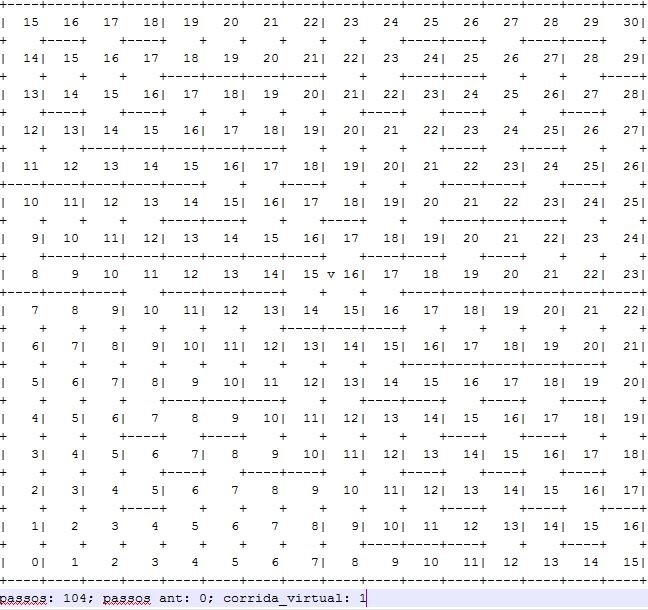
\includegraphics[width=0.5\linewidth]{seol01_4.JPG}
	\end{center}
	\centering
	\small Fonte: autor (2017)
\end{figure}
\begin{figure}[!htb]
	\caption{\label{fig:seoul01_6}Atualização das distâncias das células para o robô voltar à celula de partida - corrida virtual 3}
	\begin{center}
		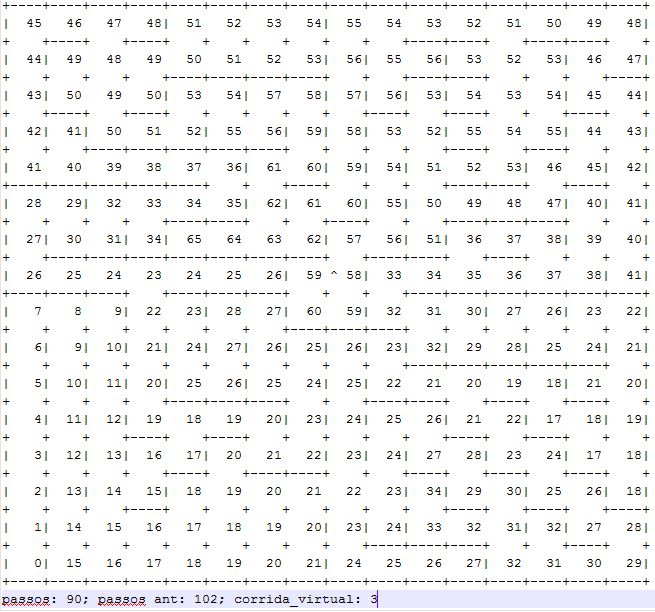
\includegraphics[width=0.5\linewidth]{seol01_6.JPG}
	\end{center}
	\centering
	\small Fonte: autor (2017)
\end{figure}

\begin{figure}[!htb]
	\caption{\label{fig:seoul01_7}Atualização das distâncias das células para o robô voltar à celula de partida - corrida virtual 5}
	\begin{center}
		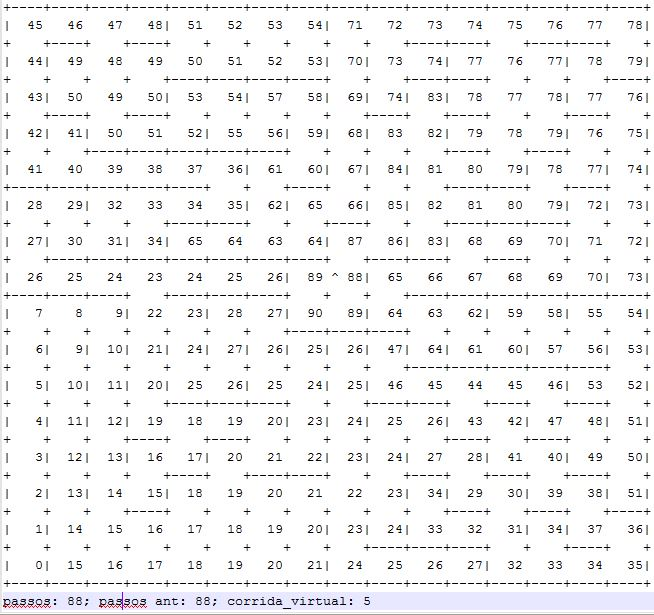
\includegraphics[width=0.5\linewidth]{seol01_7.JPG}
	\end{center}
	\centering
	\small Fonte: autor (2017)
\end{figure}


\begin{figure}[!htb]
	\caption[Labirinto \emph{Seoul} após 3 corridas \emph{reais}]{\label{fig:seoul01_8}Labirinto Seoul após 3 corridas reais}
	\begin{center}
		\subfloat[Algoritmo proposto]{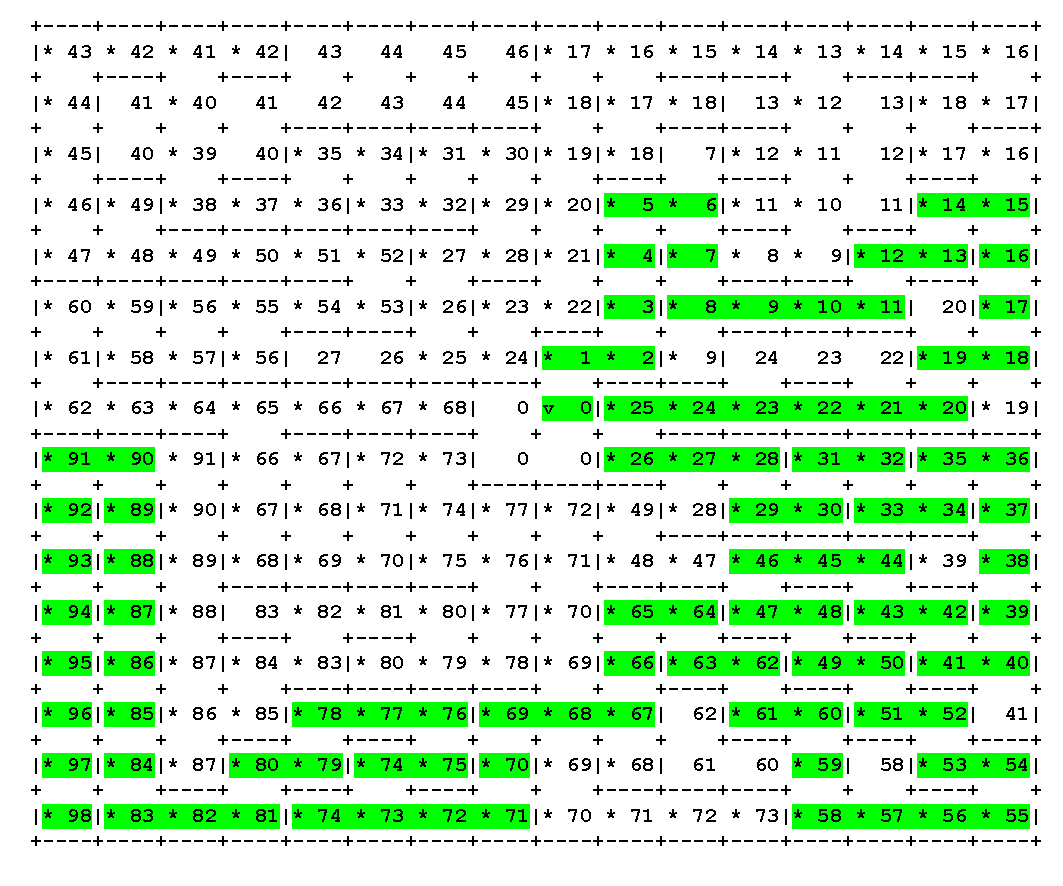
\includegraphics[width=0.45\linewidth]{seol01_8.pdf}}
		\hspace*{0.1\linewidth}
		\subfloat[Simulador Micromouse]{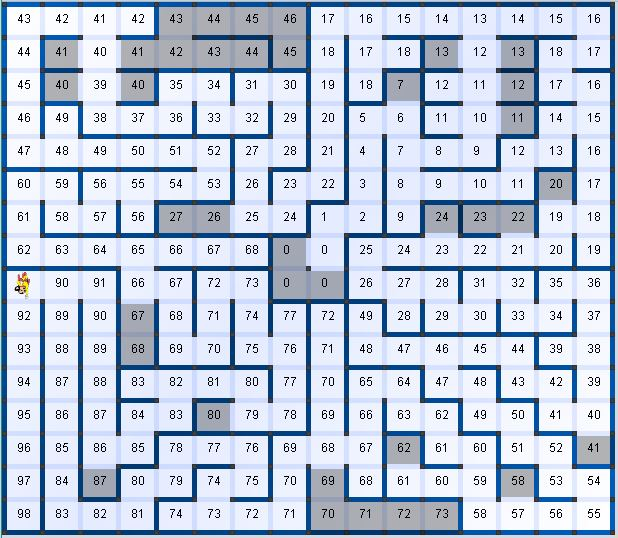
\includegraphics[width=0.4\linewidth]{seol01_9.JPG}}
	\end{center}
	\centering
	\small Fonte: autor (2017)
\end{figure}

A eficiência do algoritmo permanece intacta. Após 3 corridas \emph{reais}, tanto o algoritmo proposto como o algoritmo do simulador \emph{Micro Mouse Maze Editor and Simulator} apresenta a mesma distribuição dos números das células, como mostram as Figuras \ref{fig:seoul01_8} (a) e \ref{fig:seoul01_8} (b). O percurso otimizado está em verde.

Algumas estatísticas foram feitas para os algoritmos \emph{Flood Fill}, expostas na Tabela \ref{tab:estatistica1}, onde pode-se perceber que há algumas diferenças, para o mesmo labirinto. No entanto, o número de células visitadas para a melhor corrida permanece o mesmo. Estas diferenças podem ser explicadas. Para decisões de sentido para vizinhanças de mesmo número, a prioridade para o sentido é diferente.


%algoritmo no maze seoul 01

\begin{table}[!htb]
	\centering
	\caption{\label{tab:estatistica1}Desempenho dos algoritmos no labirinto \emph{Seoul}}
\begin{tabular}{c|cc}
\textbf{Estatísticas} & \textbf{Algoritmo proposto}  & \textbf{\emph{Micro Mouse}} \\ 
\hline 
\textbf{Únicas células atravessadas} & 224 & 218 \\ 
\hline 
\textbf{Cél. p/ chegar ao centro (1$^a$ vez)} & 293 & 292\\ 
\hline 
\textbf{Curvas (na primeira corrida)} & 164 & 164\\ 
\hline 
\textbf{Células visit. na melhor corrida} & 98 &  98\\ 
\hline 
\textbf{Curvas (melhor caminho)} & 60 & 60 \\ 
\hline 
\textbf{Cél. atrav. p/ comp. a melhor corrida} & 695 & 694 \\ 
\hline 
\textbf{Curvas (p/ completar a melhor corrida)} & 388 & 398 \\ 
\end{tabular} 
	
	\legend{Fonte: autor (2017)}
\end{table}


%
%\begin{figure}[!htb]
%	\caption{\label{fig:seoul01_8}Labirinto \emph{Seoul} após 3 corridas \emph{reais}}
%	\begin{center}
%		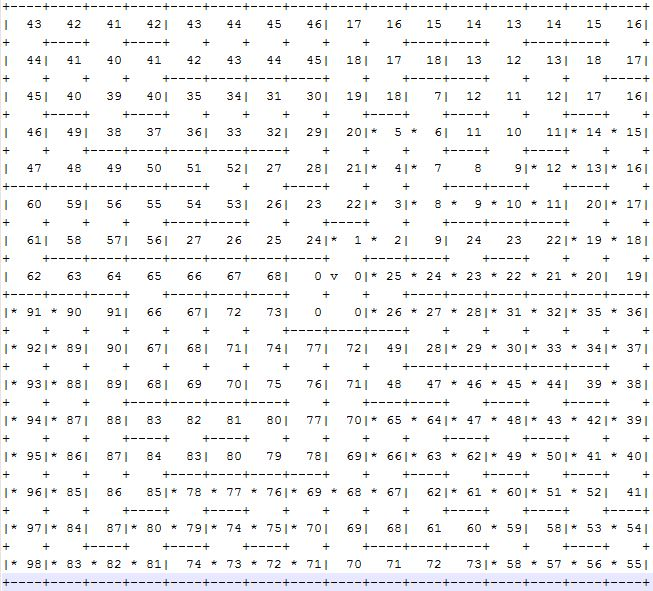
\includegraphics[width=1.0\linewidth]{seol01_8.JPG}
%	\end{center}
%	\centering
%	\small Fonte: do autor
%\end{figure}
%
%\begin{figure}[!htb]
%	\caption{\label{fig:seoul01_9}Labirinto \emph{Seoul} após 3 corridas \emph{reais} no \emph{Micro Mouse Maze Editor and Simulator}}
%	\begin{center}
%		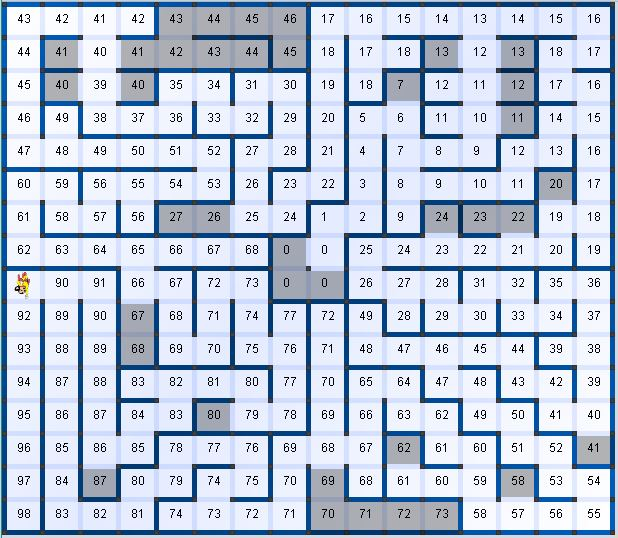
\includegraphics[width=1.0\linewidth]{seol01_9.JPG}
%	\end{center}
%	\centering
%	\small Fonte: do autor
%\end{figure}


\section{Controle em malha fechada do Micromouse}
O controle proposto por \citeonline{6734188} foi implementado na plataforma Simulink, utilizando as funções de transferência \texttt{G(z)} dos motores estimados pelo \emph{Método dos Mínimos Quadrados Não Recursivos} e os parâmetros PID estimados pelo \emph{Método sequencial do relé}.

Como referência para os controladores, um bloco chamado \emph{Repeating Sequence Interpolated} permite a inserção de vetores de saída e vetores com valores de tempo; os perfis de curva e de reta poderão ser modelados por este bloco. A determinação destes vetores será mostrado adiante. Portanto, pode-se verificar a robustez dos controladores e, ao mesmo tempo, o percurso do micromouse num plano cartesiano.

Após as simulações, o controlador digital realimentado proposto foi implementado no Micromouse, com os mesmos parâmetros PID determinados pelo método do relé em simulação. Outra máquina de estados foi criada, com o objetivo de fornecer sinais de referência para os controladores. Enquanto o robô percorria o labirinto, as referências geradas de velocidades linear e angular para os controladores, as variáveis de controle e de saída eram enviadas para o \textit{MATLAB}, de forma \emph{online}, por conexão \textit{bluetooth}, e gráficos foram gerados para validação do sistema de controle como todo.

\subsection{Simulação do processo motor-\textit{encoder}}

A simulação do controle de Figura \ref{fig:mimo_pid} foi construído no Simulink, com objetivo de testar os perfis de curva e de velocidade. Os controladores de velocidades devem ser bons rastreadores de referência, de forma a estabilizar as saídas para entradas de referência em degrau e em rampa. 

Os coeficientes estimados pelo Método dos Mínimos Quadrados foram postos via \emph{bloco de função de transferência discreta} para emular os motores do Micromouse.

Os parâmetros do bloco PID foram extraídos a partir do Método do relé sequencial em simulação, e, posteriormente, foi incorporada uma parte que mostra a trajetória do ponto do centro geométrico do robô num plano XY.

\subsubsection{Método do relé sequencial para sintonia do controlador PID}

O Método do relé sequencial é um ótimo sintonizador. A técnica para sintonia do sistema MIMO é bem prática e simples. A Figura \ref{fig:controle_simulink_rele} mostra o esquema feito para sintonia do Método do relé sequencial. Nas duas malhas, os relés ficam disponíveis para oscilar o sistema, caso as chaves os selecionam. Para ambos os relés, a histerese escolhida é de $\varepsilon=10$, e $d = 250$.

\begin{figure}[!h]
	\caption{\label{fig:controle_simulink_rele}Diagrama de blocos do Método do relé sequencial para o sistema MIMO proposto}
	\begin{center}
		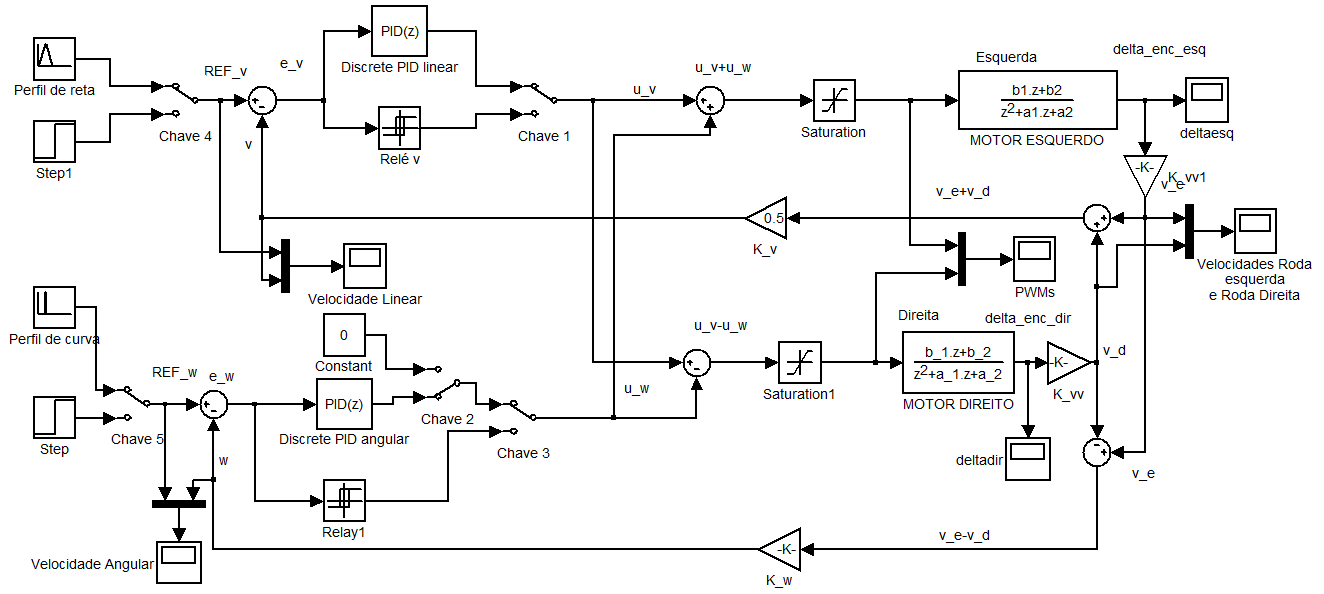
\includegraphics[width=1\linewidth]{rele_seq_sim.png}
	\end{center}
	\legend{Fonte: autor (2017)}
\end{figure}

Então, para a primeira sequência, a chave 1 da Figura \ref{fig:controle_simulink_rele} selecionou o relé para a malha de velocidade linear, e a malha de velocidade angular ficou em aberto (Chave 2 e Chave 3 selecionam o bloco de constante zero). As chaves 4 e 5 ativaram os blocos \emph{step} configurados para valor final de $50~cm/s$ e $100~^o/s$, respectivamente, para as malhas de velocidade linear e angular. Calculou-se os parâmetros PID com o método do relé SISO, através dos parâmetros do relé e do sinal de velocidade linear. Os sinais do relé e de saída, além do ponto do ganho crítico $G_v(j\omega)$ de \emph{Nyquist} para a malha de velocidade, podem ser observados na Figura \ref{fig:teste_rele_seq1}. Após, a Chave 1 seleciona o bloco PID com os parâmetros calculados pela tabela do Ziegler-Nichols.


Seguindo a sequência, configurando a chave 3, o relé da malha de velocidade angular é selecionado, de forma que o sinal fornecido por ele interfira em ambas as malhas. Calcula-se os parâmetros PID do bloco, a partir do sinal de velocidade angular de saída, e o seleciona para controlar a malha da velocidade angular. 

\begin{figure}[!htb]
	\caption{\label{fig:teste_rele_seq1}Relé na malha de velocidade linear}
	\begin{center}
		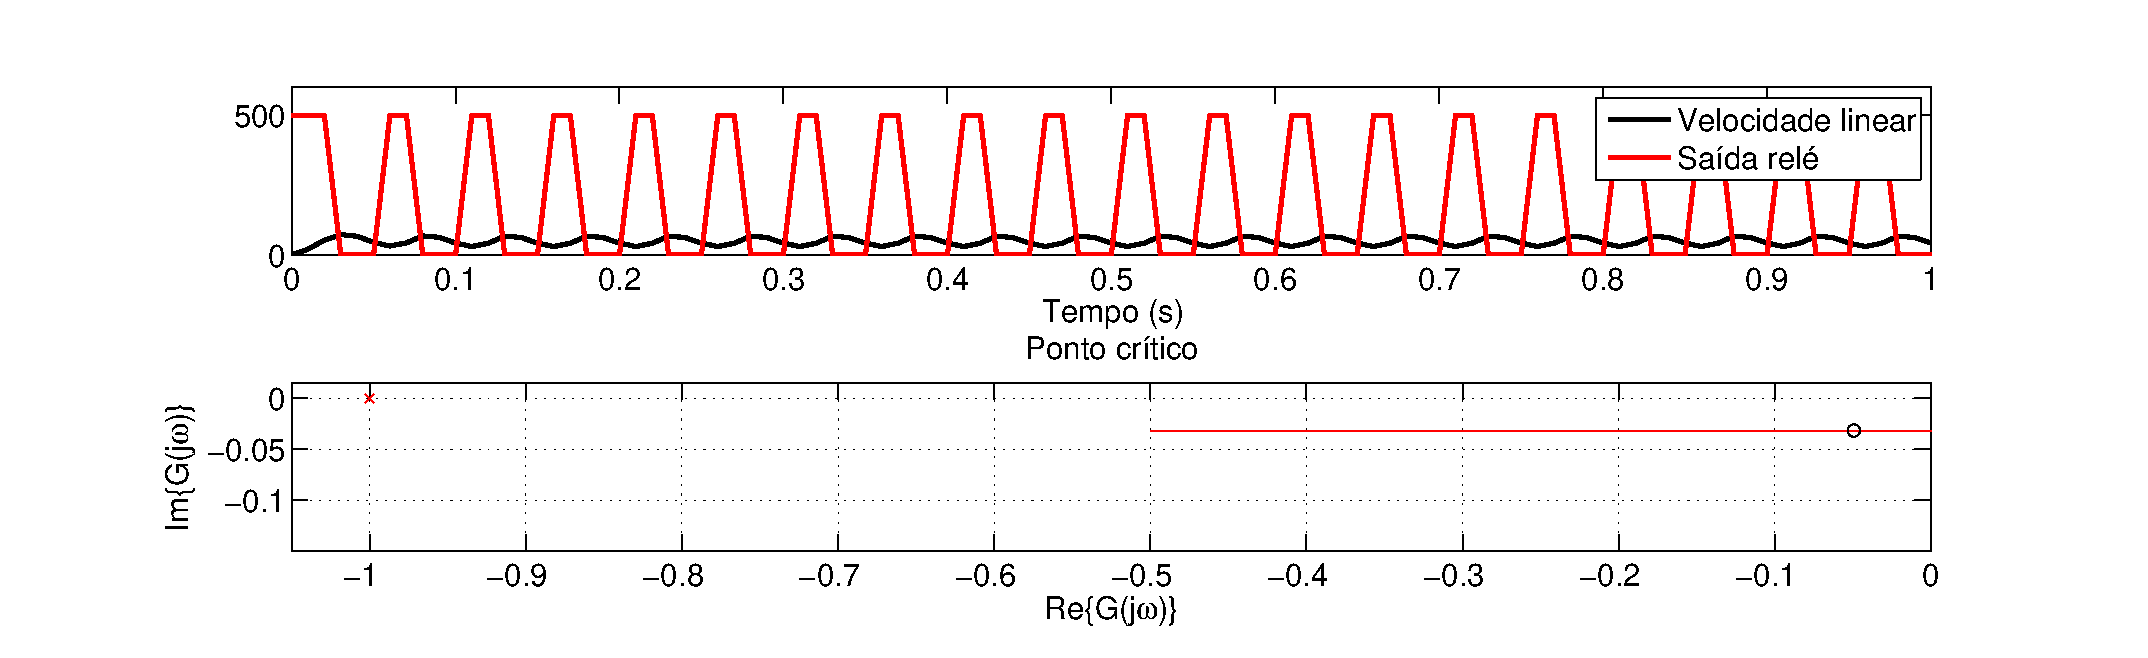
\includegraphics[width=1\linewidth]{saida_rele_linear_simul.eps}
	\end{center}
	\legend{Fonte: autor (2017)}
\end{figure}

Os sinais do relé e de saída de velocidade angular, além do ponto do ganho crítico $G_\omega(j\omega)$ de \emph{Nyquist} para esta malha, podem ser observados na Figura \ref{fig:teste_rele_seq2}.

\begin{figure}[!htb]
	\caption{\label{fig:teste_rele_seq2}Relé na malha de velocidade angular}
	\begin{center}
		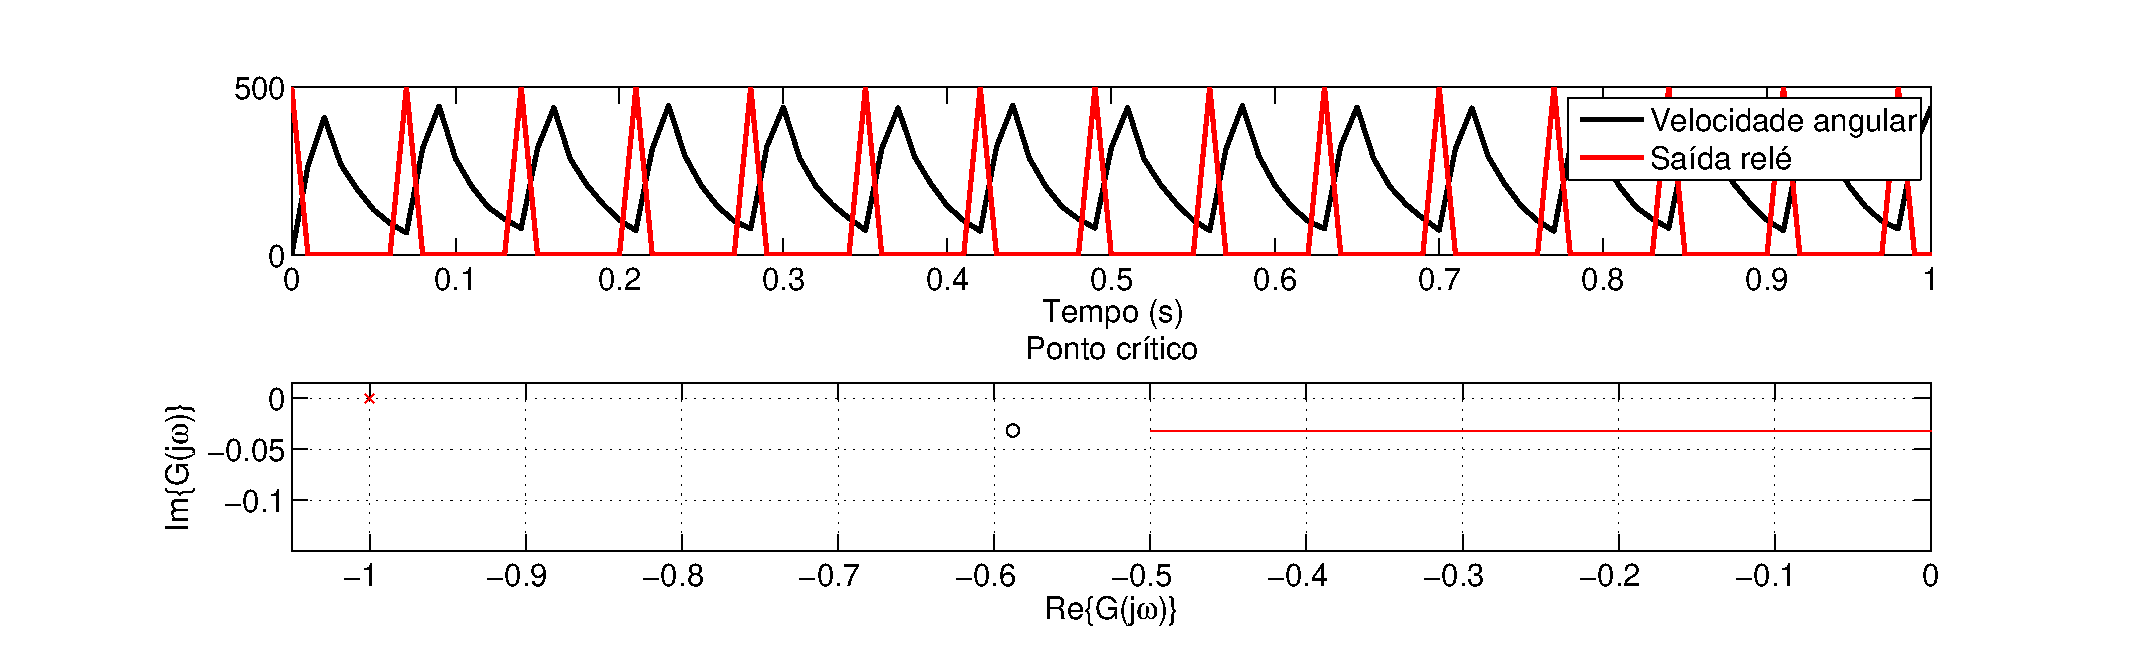
\includegraphics[width=1\linewidth]{saida_rele_ang_simul.eps}
	\end{center}
	\legend{Fonte: autor (2017)}
\end{figure}

Este processo foi repetido até que não houvesse mais mudanças nos valores parâmetros dos controladores. Os processos, cujo $K_pK_u$ estando entre 2 e 20, podem ser controlados pelos blocos PID sintonizados a partir da tabela do Ziegler-Nichols \cite{COELHO:2015}. A Tabela \ref{tab:k_u2} mostra algumas grandezas críticas obtidas a partir do método. A Tabela \ref{tab:PID_siso_simulador} mostra os valores dos parâmetros PID para ambos os controladores do sistema MIMO. Comparando os pontos de ganho crítico $G_v(j\omega)$ e $G_\omega(j\omega)$ das malhas, a malha de velocidade é relativamente mais estável, em malha fechada, que a malha de velocidade angular.

\begin{table}[!htb]
	\centering
	\caption{\label{tab:k_u2}Dados experimentais das saídas dos processos. Foram adotados $\varepsilon=10$  e $d=250$ para ambos os relés.}
		
	\begin{tabular}{c|c|ccccc}
	\textbf{Sequência} & Malha & $a$ & $T_u (s)$ & $K_u$ & $\omega_u (rad/s)$ & $K_pK_u$\\ 
	\hline 
	\textbf{1} & V. Linear & 18.6303 & 0.05 & 20.2499 & 125.6637 & 4.9157 \\ 
	\hline 
	\textbf{2} & V. Angular & 183.2216 & 0.07 & 1.7399 & 89.7598 &  5.5154\\ 
	\hline
	\textbf{3} & V. Linear & 18.6337 & 0.0500 & 20.2447 & 125.6637 & 4.9211\\ 
	\hline 
	\textbf{4} & V. Angular & 183.2216 & 0.0700 & 1.7399 & 89.7598 & 5.5154\\ 
	\hline
	\textbf{5} & V. Linear & 18.6337 & 0.0500 & 20.2447 & 125.6637 & 4.9211\\ 
	\end{tabular} 
	
\legend{Fonte: autor (2017)}
\end{table}

\begin{table}[!htb]
	\centering
	\caption{\label{tab:PID_siso_simulador}Parâmetros dos blocos PID estimados pelo Método do relé sequencial em simulação}
	\begin{tabular}{c|cccc}
	Sequência & Malha & $k_P$ & $k_I$ & $k_D$ \\ 
	\hline 
	1 & V. Linear & 12.15 & 485.9985 & 0.0759 \\ 
	\hline 
	2 & V. Angular & 1.0439 & 29.8267 & 0.0091 \\ 
	\hline 
	3 & V. Linear & 12.1468 & 485.8737 & 0.0759 \\ 
	\hline 
	4 & V. Angular & 1.0439 & 29.8267 & 0.0091 \\ 
	\hline 
	5 & V. Linear & 12.1468 & 485.8737 & 0.0759 \\ 
	\end{tabular} 
	
	\legend{Fonte: autor (2017)}
\end{table}

\begin{figure}[!htb]
	\caption{\label{fig:resultado_controle_simulink_rele}Resultado da simulação do controle MIMO proposto}
	\begin{center}
		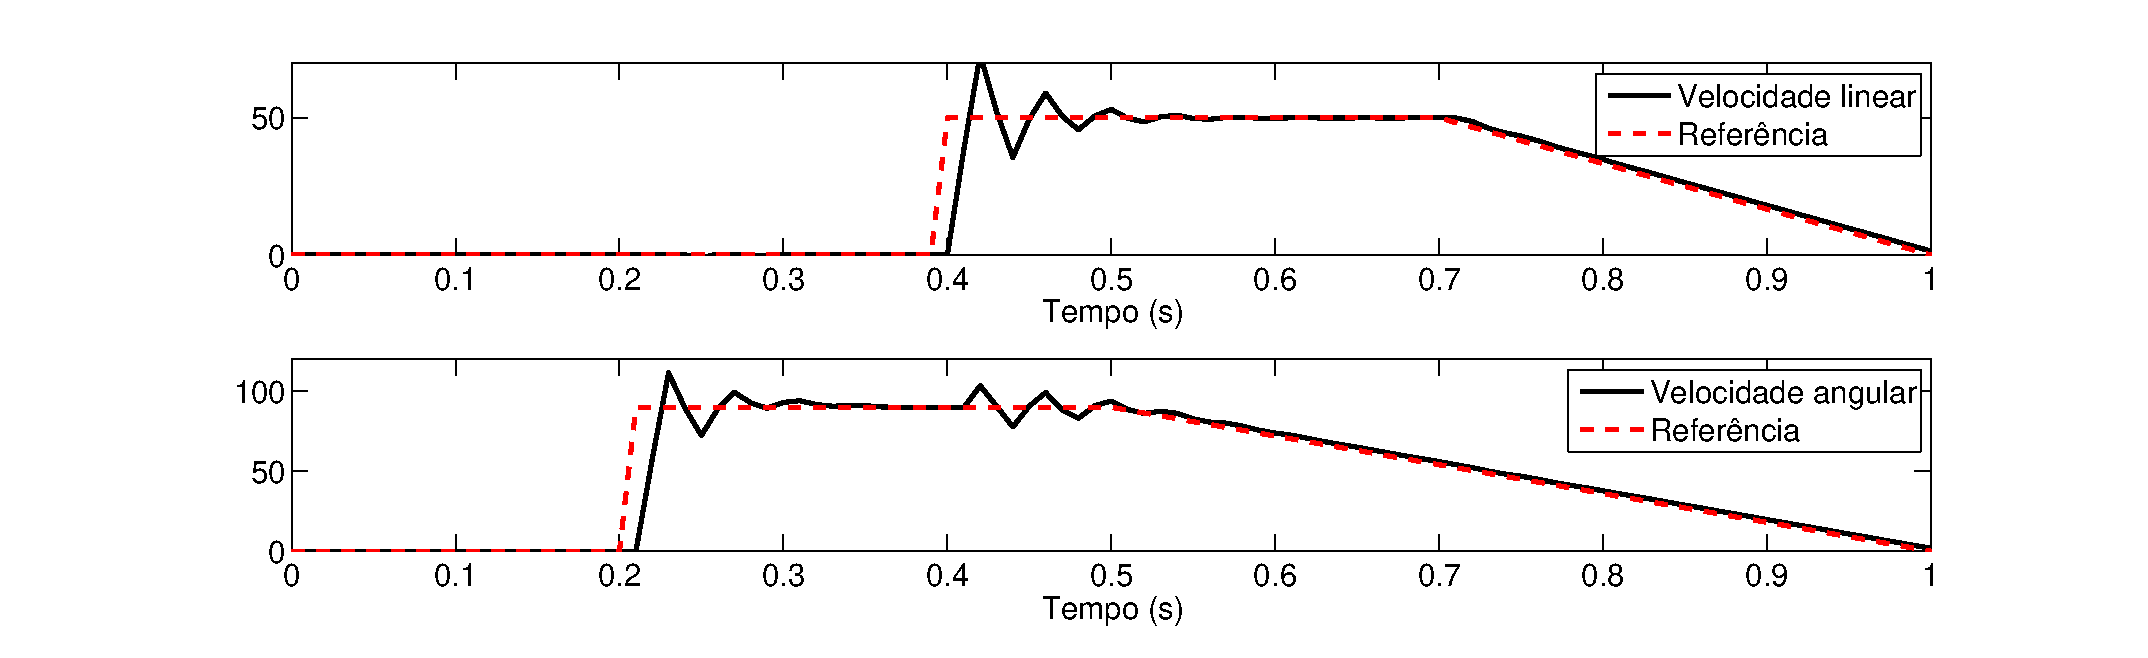
\includegraphics[width=0.8\linewidth]{resultado_simulacao.eps}
	\end{center}
	\legend{Fonte: autor (2017)}
\end{figure}


O resultado do controle de velocidade proposto já com os parâmetros PID calculados através do Método do relé sequencial pode ser observado na Figura \ref{fig:resultado_controle_simulink_rele}. As saídas seguiram corretamente as referências dos controladores, para entradas em degrau e em rampa. Pode-se perceber também que quando há uma mudança brusca de referência de velocidade angular, há uma perturbação na saída da outra malha. Os \emph{overshoots} são esperados para entradas em degrau, quando a sintonia é feita pelo método do Ziegler-Nichols. Porém, os perfis de curva e de reta são rampas de velocidade, e, portanto, os \emph{overshoots} e as interferências são mínimos, quase eliminados.


\subsubsection{Simulação das trajetórias}
Para o desenvolvimento da simulação do sistema proposto, foi implementado o sistema motor-\textit{encoder} do Micromouse no \emph{Simulink}, do \textit{MATLAB}. O esquema está na Figura \ref{fig:controle_simulink}. O modelo construído tenta aproximar-se ao sistema do Micromouse real. Os controladores utilizam os parâmetros PID da Tabela \ref{tab:PID_siso_simulador}.

\begin{figure}[!htb]
	\caption{\label{fig:controle_simulink}Diagrama de blocos do controle implementado no \textit{Simulink}}
	\begin{center}
		\includegraphics[width=1\linewidth]{controle_Micromouse.pdf}
	\end{center}
	\legend{Fonte: autor (2017)}
\end{figure}

A trajetória pode ser construída a partir da integração da velocidade linear do robô (utilizando o método trapezoidal) e do ângulo $\theta$ formado no plano cartesiano. A coordenada do Micromouse no plano XY é a própria decomposição do vetor-distância percorrida no tempo de amostragem. Em (\ref{eq:ponto_XY}) é mostrado o cálculo para depomposição do vetor-distância, num instante $k$, considerando $\theta$ em $graus$.

\begin{equation}
\label{eq:ponto_XY}
	\begin{split}
	distX(k) = (0.5 \times T_s \times (v(k) + v(k-1)) \times cos(\theta) + distX(k-1);\\
	distY(k) = (0.5 \times T_s \times (v(k) + v(k-1)) \times sin(\theta) + distY(k-1);\\
	\end{split}
\end{equation}

Os vetores dos perfis de reta e de curva utilizados na simulação foram calculados conforme (\ref{eq:traj_ideal}) e (\ref{eq:traj_ideal2}). O trajeto projetado faz o robô acelerar uma célula à frente, realiza uma curva para a direita e logo em seguida realiza uma curva para a esquerda e finaliza o trajeto desacelerando o robô seguindo em frente. A Figura \ref{fig:3celulas} mostra os perfis de curva e de velocidade projetados para a simulação.

\begin{figure}[!htb]
	\caption{\label{fig:3celulas}Perfis de velocidades projetados}
	\begin{center}
		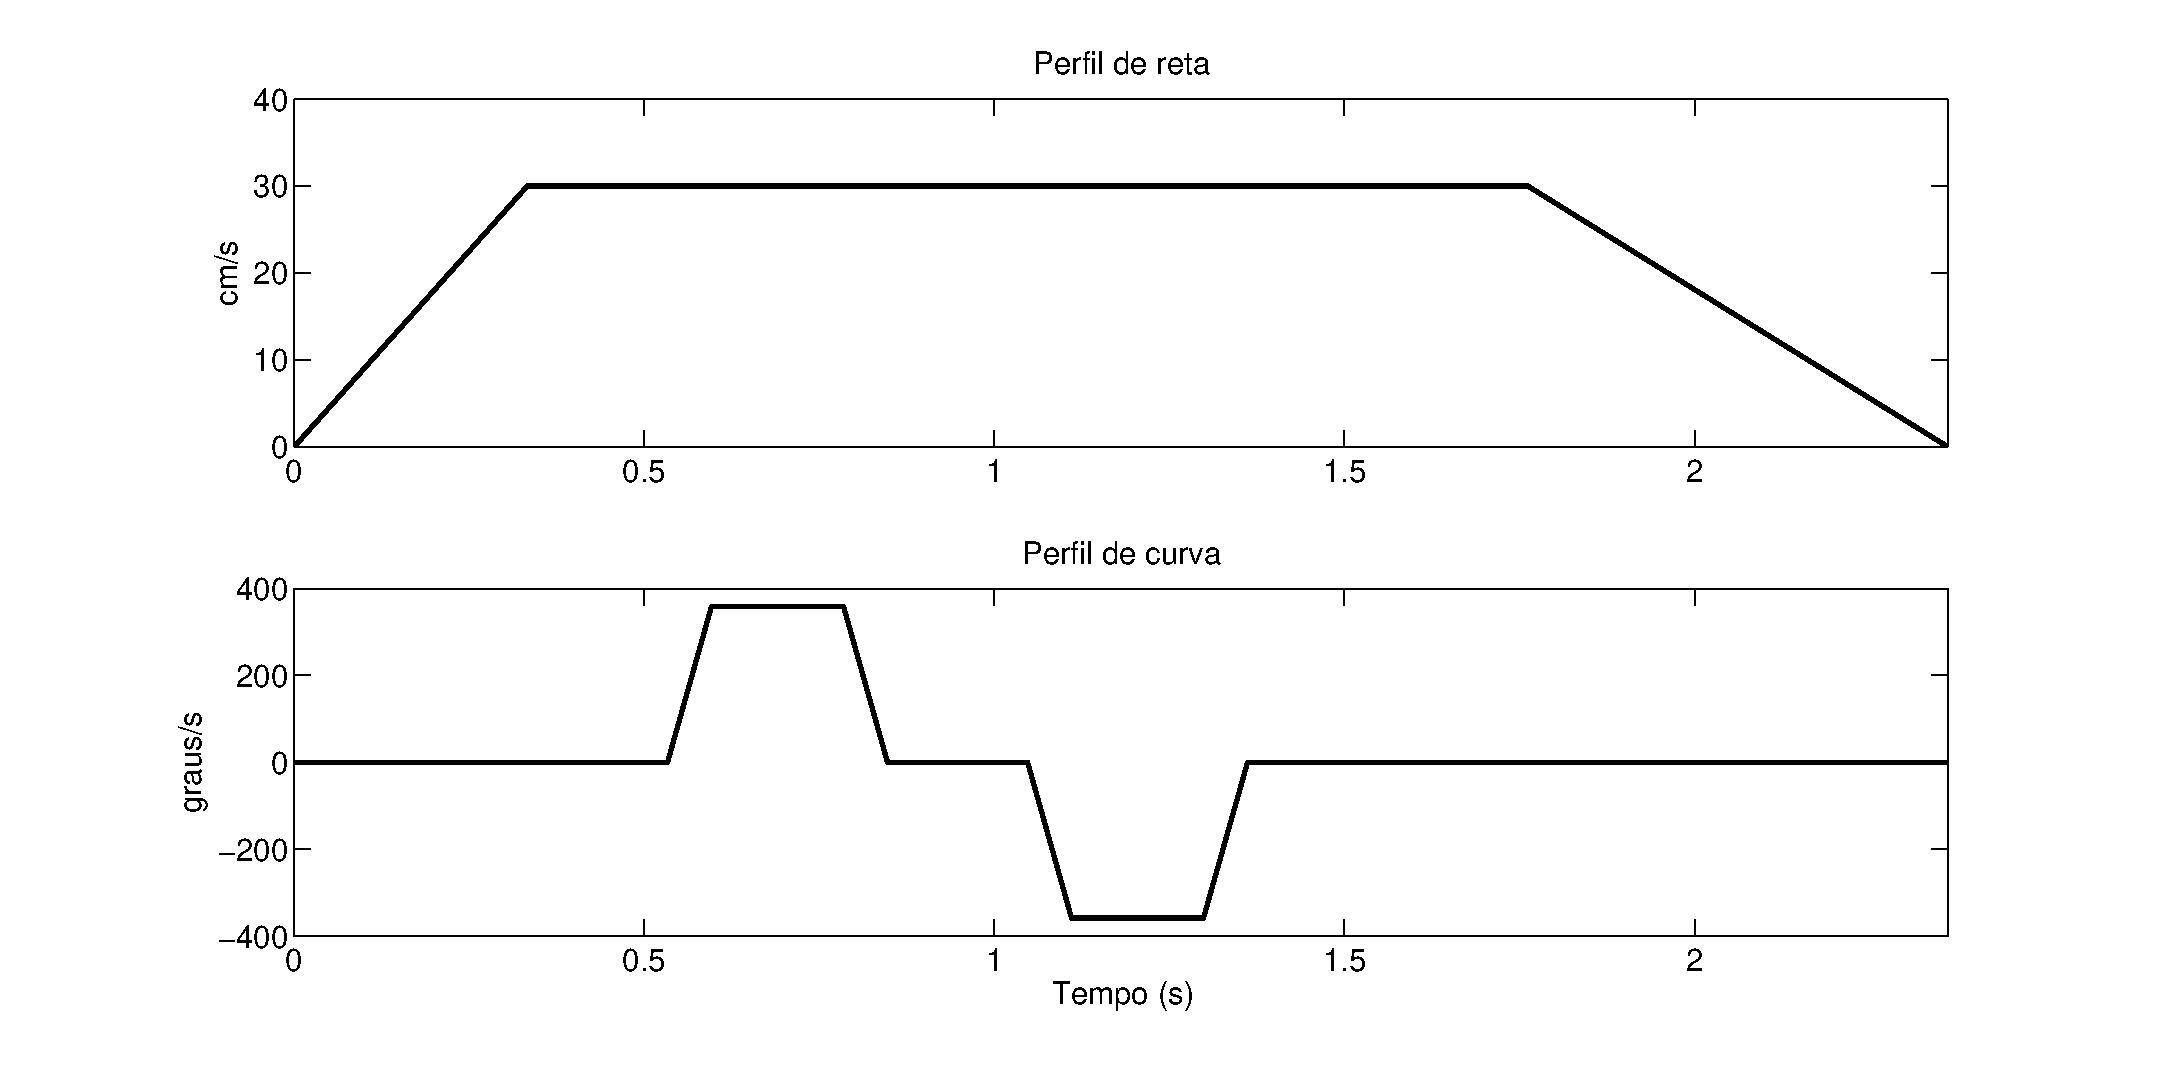
\includegraphics[width=.9\linewidth]{perfildecurva_3celulas.eps}
	\end{center}
	\legend{Fonte: autor (2017)}
\end{figure}

Dentro dos blocos que modelam os perfis de curva, foram postos os vetores de amplitude e de tempo, cujos valores estão na Tabela \ref{tab:vetores_perfis_curva}.

\begin{table}[!htb]
	\centering
	\caption{\label{tab:vetores_perfis_curva}Vetores utilizados para a simulação}
\begin{tabular}{c|cccccccc}
 & \multicolumn{7}{c}{índice} &  \\ 
\hline 
vetor & 1 & 2 & 3 & 4 & 5 & 6 & 7 & 8\\ 
\hline 
v & 0 & 30 & 30 & 30 & 30 & 30 & 30 & 30 \\ 
w & 0 & 0 & 0 & 0 & 358 & 358 & 0 & 0 \\ 
\hline 
tempo & 0 & 0.333 & 0.7667 & 0.8667 & 0.9295 & 1.118 & 1.180 & 1.2808\\ 
\hline 
 & \multicolumn{7}{c}{índice} & \\ 
\hline 
vetor & 9 & 10 & 11 & 12 & 13 & 14 & 15 &\\ 
\hline 
v & 30 & 30 & 30 & 30 & 30 & 30 & 0 &\\ 
w & 0 & -358 & -358 & 0 & 0 & 0 & 0 &\\ 
\hline 
tempo & 1.3808 & 1.4437 & 1.6322 & 1.695 & 1.795 & 2.095 & 2.696 &\\ 
\end{tabular} 
	\legend{Fonte: autor (2017)}
\end{table}
O resultado da simulação ocorreu conforme o esperado. A trajetória desenhada perfeita das curvas e retas, como mostra a Figura \ref{fig:resultado_trajetoria}, prova que o sistema de controle e os perfis de velocidade trabalham satisfatoriamente. 

\begin{figure}[!htb]
	\caption{\label{fig:resultado_trajetoria}Simulação da trajetória do robô utilizando os perfis de velocidade como referência para o controlador}
	\begin{center}
		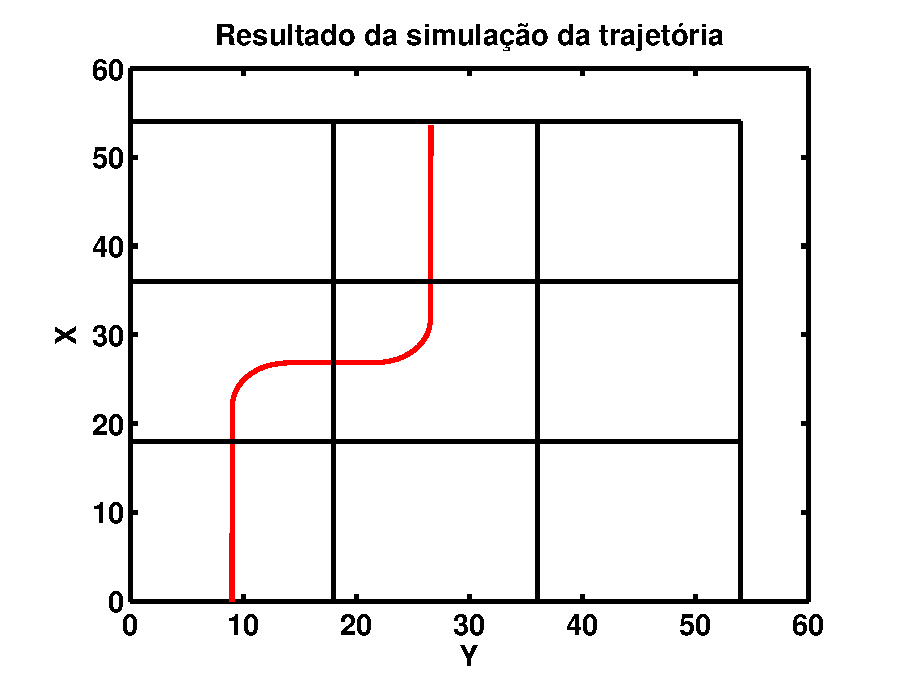
\includegraphics[width=.7\linewidth]{resultado_trajetoria.eps}
	\end{center}
	\legend{Fonte: autor (2017)}
\end{figure}

Então, o robô pôde ser automatizado por completo utilizando o algoritmo \emph{Flood Fill} e os perfis de curva e de reta projetados para os quatro estados do algoritmo. 


\begin{figure}[!htb]
	\caption{\label{fig:resultado_controle_trajetoria}Perfis de velocidade e sinais de saída do controlador proposto}
	\begin{center}
		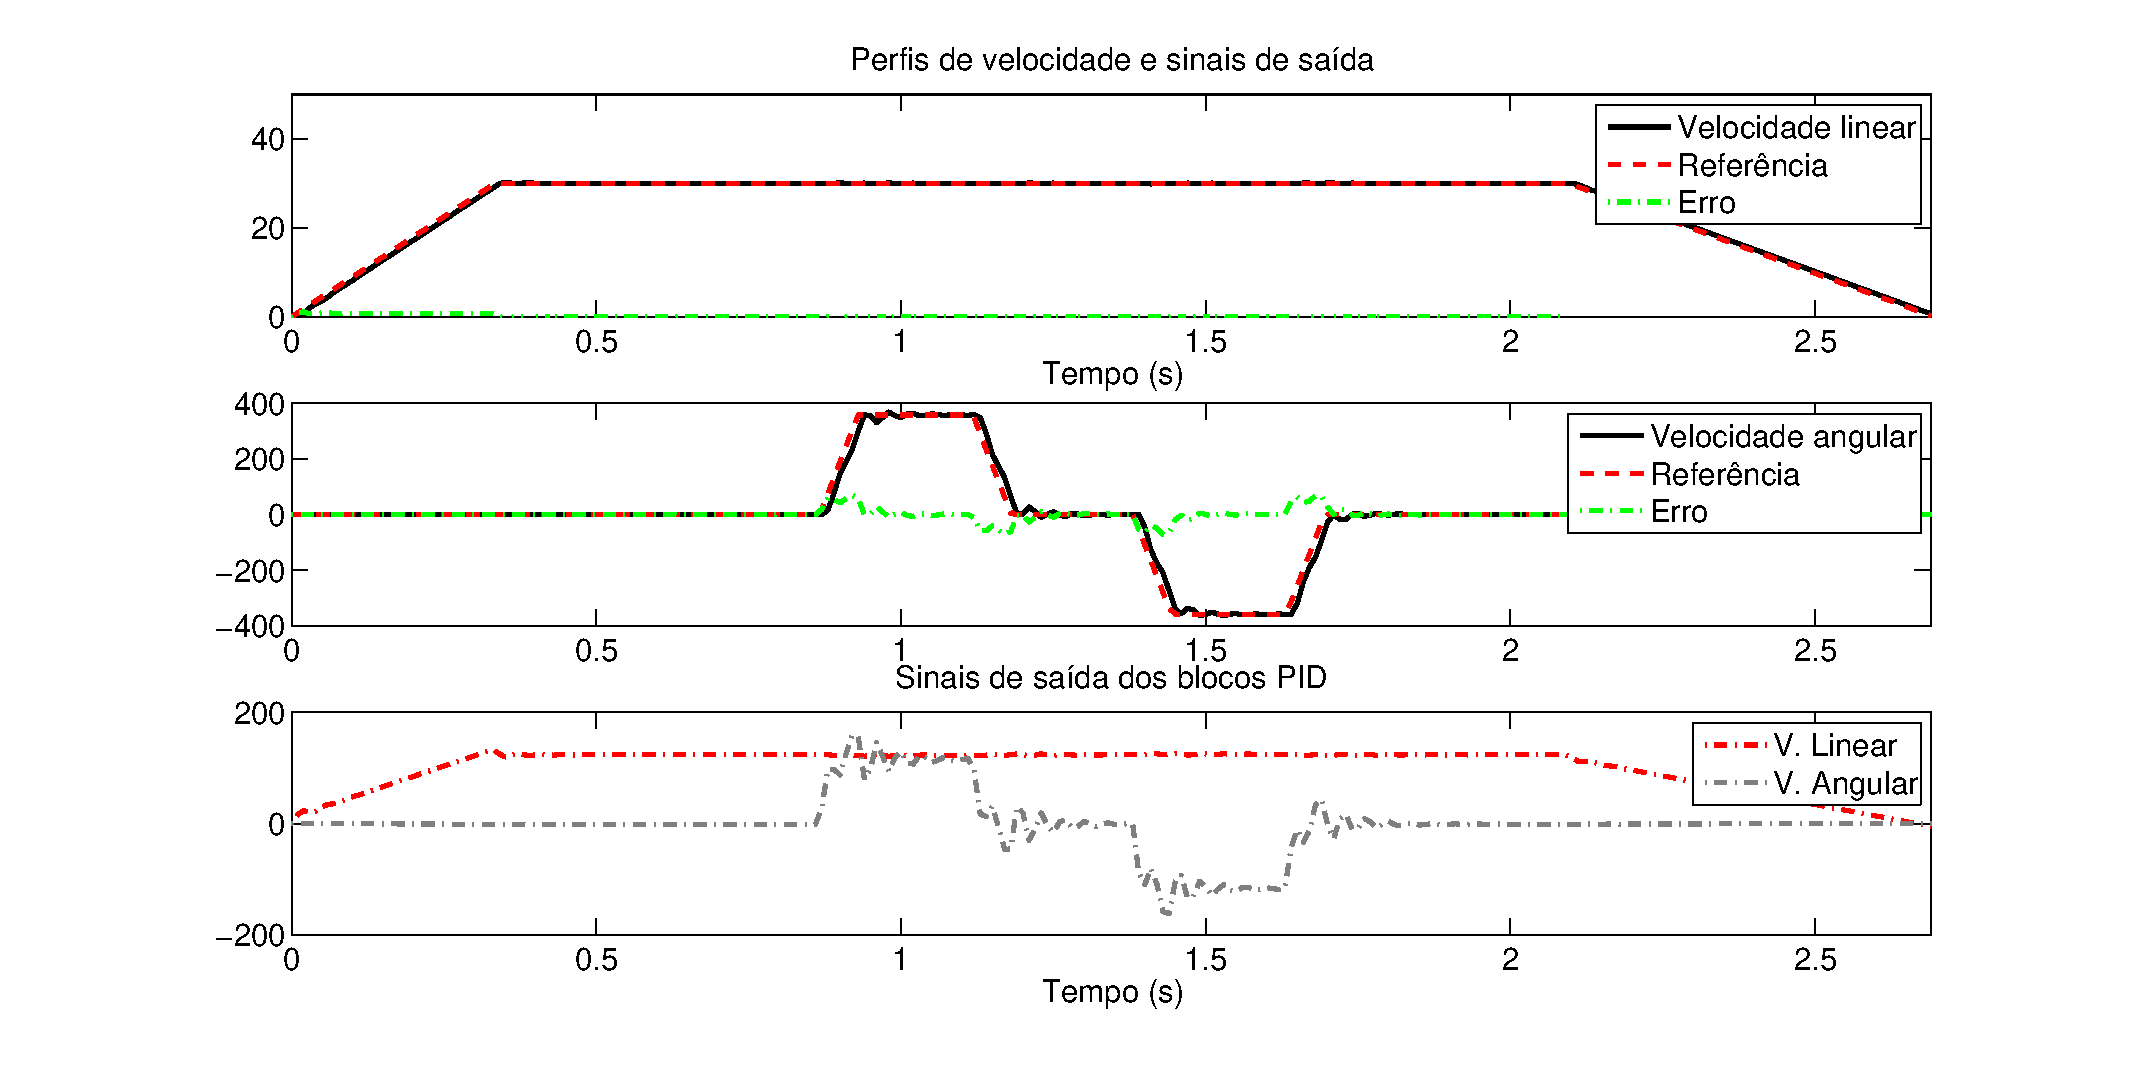
\includegraphics[width=.9\linewidth]{resultado_controle_trajetoria.eps}
	\end{center}
	\legend{Fonte: autor (2017)}
\end{figure}

O erro de rastreamento, como pode ser observado na Figura \ref{fig:resultado_controle_trajetoria}, é praticamente nulo. Como as entradas são rampas, os \emph{overshoots} são praticamente eliminados. Os sinais de controle gerados pelos controladores PID sintonizados pelo método sequencial do relé também é mostrado. Mesmo com a variação da referência de velocidade angular, a velocidade linear praticamente não foi afetada, mostrando a estabilidade da malha de velocidade linear.


\subsection{Aplicando o controle no mini-robô Micromouse}

A discretização de um controlador PID analógico (\ref{eq:pid}) pode ser feita de diversas maneiras. Um dos métodos de discretização é a já conhecida aplicação da transformada Z à função analógica discretizada. Para o Micromouse em questão, foi utilizada a discretização por meio da integração trapezoidal. O PID discretizado está em (\ref{eq:PID_discret}). Os parâmetros PID utilizados foram os da Tabela \ref{tab:PID_siso_simulador}.

\begin{equation}
\label{eq:PID_discret}
	\begin{split}
		&e(t) = REF - y(t) \\
		&u_P(t) = K_P \times e(t)\\
		&u_I(t) = K_I \times T_s \times 0.5 \times (e(t) + e(t-1)) + u_I(t-1)\\
		&u_D(t) = K_D \times (e(t) - e(t-1))/T_s\\
		&u_{PID}(t) = u_P(t) + u_I(t) + u_D(t)\\
	\end{split}
\end{equation}

	Porém, como o Micromouse carece de RAM, utilizou-se somente uma variável para cada termo do PID ao invés de um \emph{array}. Desta forma, os dois controladores PID foram implementados. O trecho do controle MIMO implementado mostra a equação dos dois controladores de forma otimizada:
\begin{verbatim}
		e_v = REF_v - v; 
		u_P = K_P * e_v; 
		u_I = K_I * T_s *0.5 * (e_v + e_v_ant) + u_I; 
		u_v = u_P + u_I + u_D;
		e_w = REF_w - w;
		u_Pw = K_Pw * e_w;
		u_Iw = K_Iw * T_s * 0.5 * (e_w + e_w_ant) + u_Iw;
		u_Dw = K_Dw * (e_w - e_w_ant)/T_s;
		u_w = u_Pw + u_Iw + u_Dw;
		e_v_ant = e_v;
		e_w_ant = e_w;
\end{verbatim}

	O resultado da implementação do controlador PID na malha de velocidade linear está na Figura \ref{fig:resultado_controle_micromouse}. 
	
\begin{figure}[!htb]
	\caption{\label{fig:resultado_controle_micromouse}Resultado do controle da malha de velocidade linear implementado no Micromouse}
	\begin{center}
		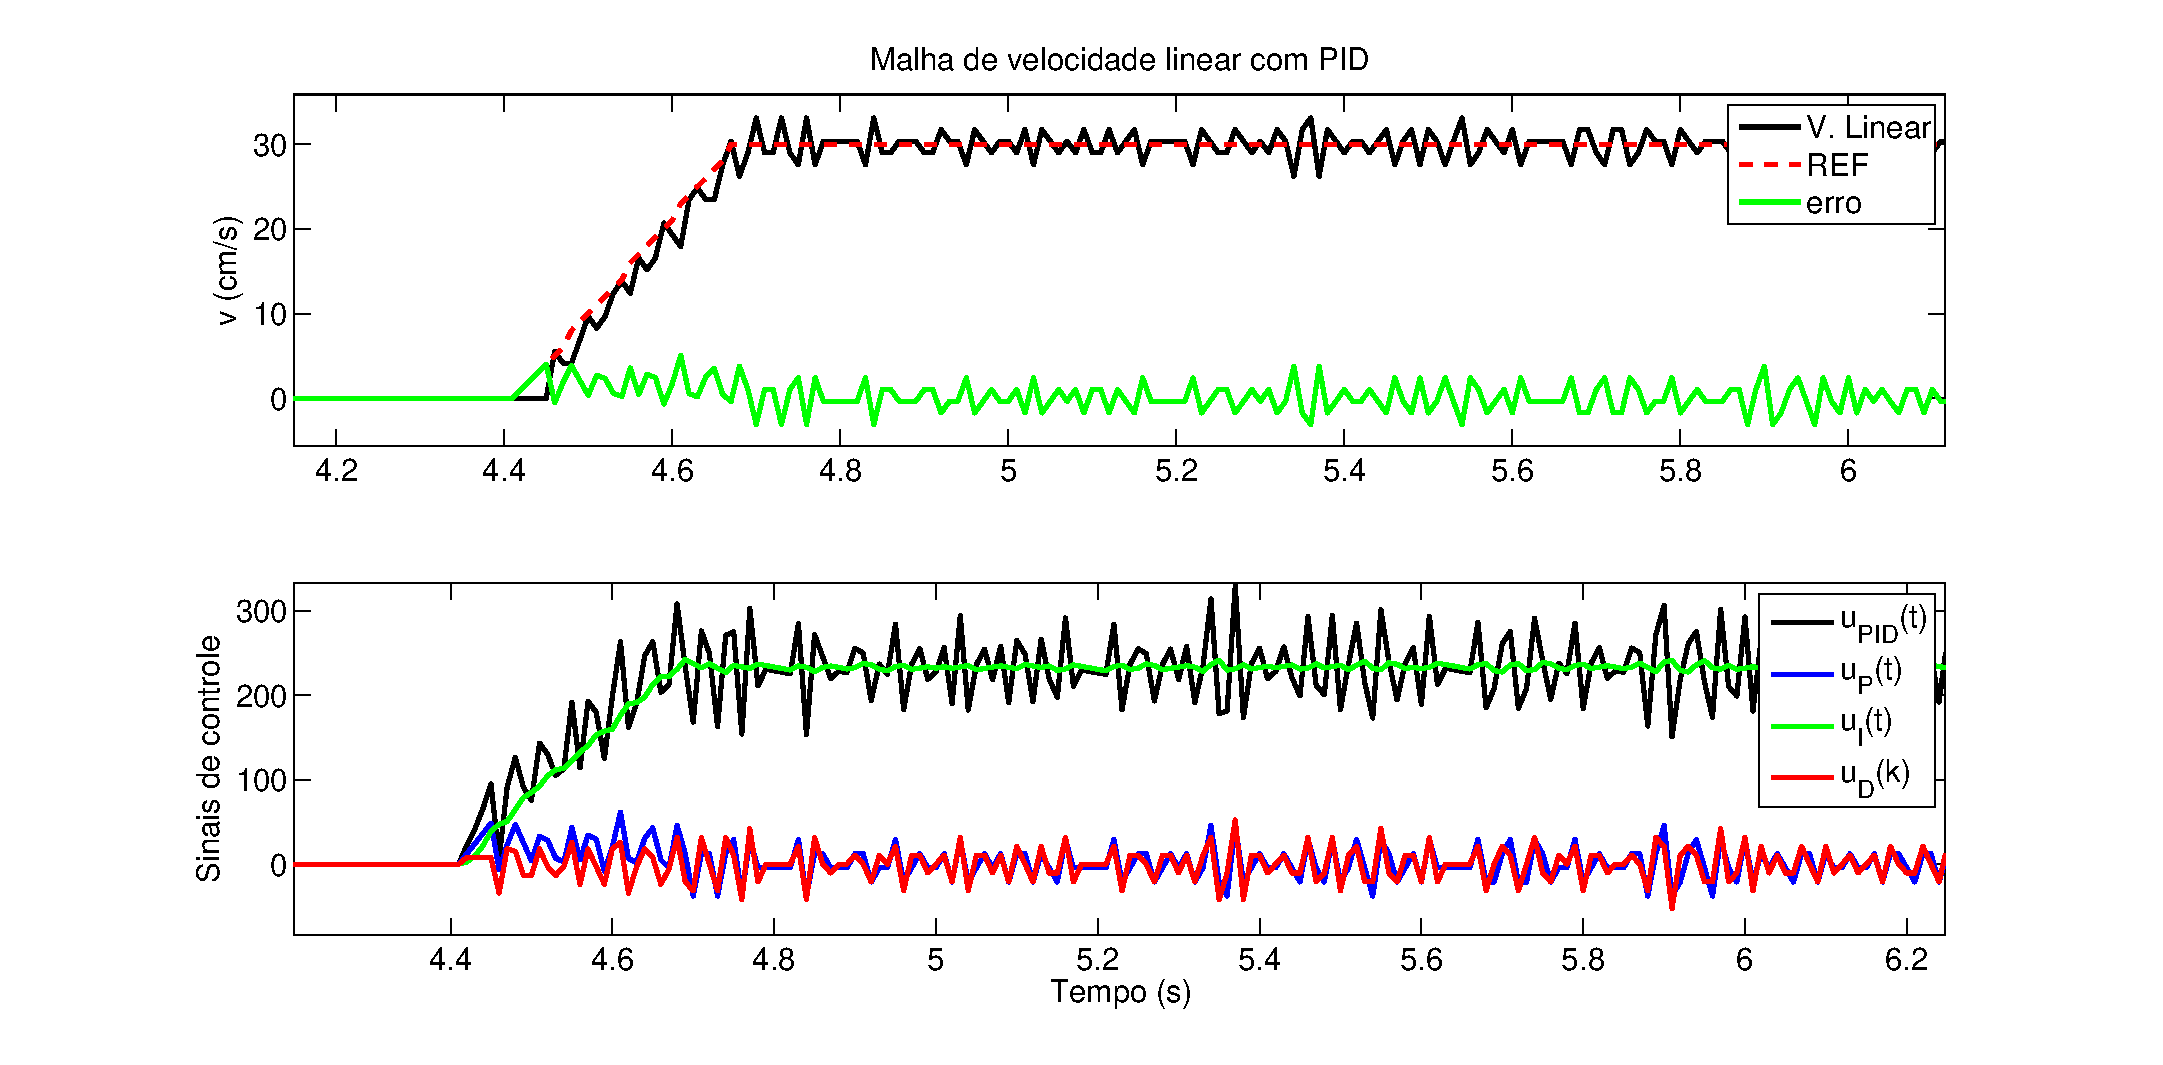
\includegraphics[width=1\linewidth]{resultado_controle_micromouse.eps}
	\end{center}
	\legend{Fonte: autor (2017)}
\end{figure}

Os ruídos comuns em sistemas reais pertubam o sinal de saída, e os controladores \emph{proporcional} e \emph{derivativo} potencializam, conforme mostra a figura, porém a média do sinal segue a referência fortemente. As entradas do tipo rampa se comportaram perfeitamente, com pouco erro de regime permanente. A curva do erro é praticamente zero. Quase não há interferência da malha de velocidade angular, mesmo com entradas em rampa. Não existiu \emph{Overshoot} característico, como previsto na simulação, para entradas em rampa.


	Já o resultado da implementação do controlador PID na malha de velocidade angular pode ser observado na Figura \ref{fig:resultado_controle_micromouse2}. As oscilações comuns devido ao ruído, potencializados pelos controladores proporcional e derivativo, como pode ser observado o nível do sinal dos mesmos na figura, acabam deixando o sinal sujo, porém, a média do sinal segue firme a referência. O erro é baixo para a malha de velocidade linear, com erro máximo absoluto de $5~cm/s$, porém, para velocidade angular, o erro máximo absoluto atingiu o valor de $100~^o/s$, sendo $\omega_{max}$ igual a $358~^o/s$. Portanto, a sintonia de processos MIMO pelo Método do relé sequencial logrou êxito, para velocidades baixas. Para maiores velocidades tangenciais, o erro absoluto torna-se maior para a velocidade angular, isto porque, para mesmo raio de curvatura, a velocidade angular máxima $\omega_{max}$ aumenta proporcionalmente, forçando uma aceleração mais abrupta.
	


	O robô poderá utilizar os parâmetros sintonizados, porém, para diminuir as oscilações devido ao ruído iminente do sistema motor-rodas, um \emph{ajuste fino} foi feito no ganho derivativo dos controlador da malha de velocidade angular, e seu valor foi diminuído para 70\% do valor original, o que melhorou um pouco a sua saída.
	
\begin{figure}[!htb]
	\caption{\label{fig:resultado_controle_micromouse2}Resultado do controle da malha de velocidade angular implementado no Micromouse}
	\begin{center}
		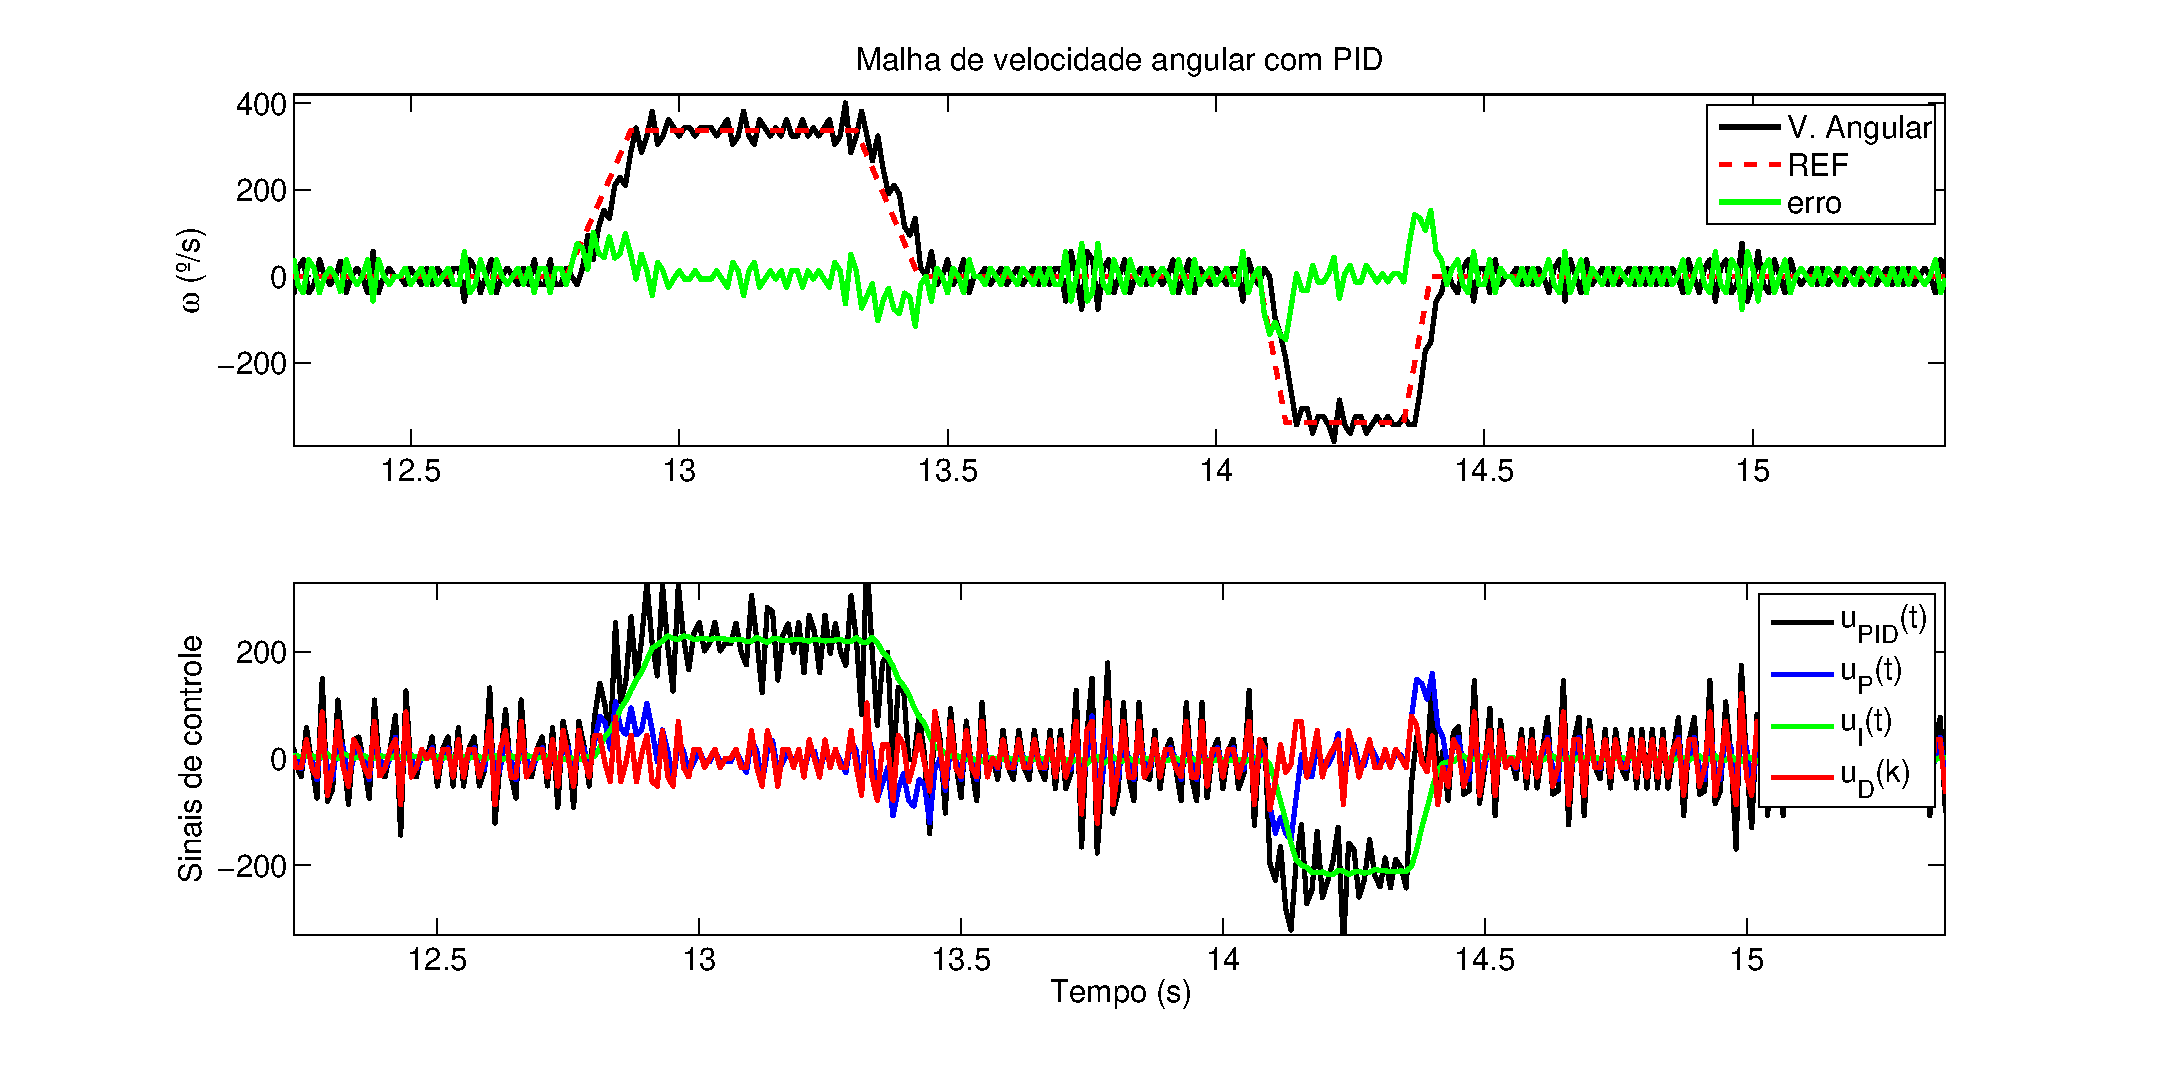
\includegraphics[width=1\linewidth]{resultado_controle_micromouse2.eps}
	\end{center}
	\legend{Fonte: autor (2017)}
\end{figure}


	Portanto, a sintonia via método do relé é simples e funcional. À frente, é mostrado resultado da união das partes implementadas num labirinto-teste.

\section{Sistema completo}

Todas as partes de \textit{hardware} e de \textit{software} são importantes para um bom desempenho do Micromouse. Através do \textit{ECLIPSE IDE}, foi gravado o programa \emph{Flood Fill}, já em linguagem C, em conjunto com o sistema de controle para velocidades, de forma que o robô possa se locomover pelo labirinto de forma autônoma e inteligente. Portanto, os primeiros resultados foram obtidos para labirinto de 8$\times$8 e, posteriormente, para o labirinto completo.

Após as implementações das partes e simulações, foram feitas as junções das mesmas. O programa do algoritmo \emph{Flood Fill}, criado já na linguagem padrão de gravação do microcontrolador, foi repassado para o programa \textit{ECLIPSE IDE} quase sem modificação. A parte do algoritmo que atualizava as paredes para modelagem do labirinto e emulava os sensores das paredes foi retirado. 

Primeiro, realizou-se o teste do programa \emph{Flood Fill} no Micromouse a fim de verificar o funcionamento do algoritmo embarcado no microcontrolador. O robô não se movimentava fisicamente. O passo era garantido com o aperto do botão. A cada aperto, o robô dava um passo e imprimia o labirinto visto pelo robô, via \textit{bluetooth}, para um terminal de porta serial. 

Também, foi possível avaliar a função de detecção das paredes. Posteriormente à implementação de todas as partes no código do Micromouse, no estado \verb+IMPRIMIR_MAZE+, a função responsável por exibir o labirinto visto pelo robô foi desativado e a validação dos testes passou a ser feita de forma visual, sobre o labirinto.

Os primeiros testes foram feitos no labirinto com poucas paredes, como é mostrada na Figura \ref{fig:labteste}. O objetivo era testar os perfis de curva e a função para detecção das paredes, isto já com o algoritmo \emph{Flood Fill} para indicar o sentido.

\begin{figure}[!htb]
	\caption{\label{fig:labteste}Foto do primeiro teste do Micromouse sobre o tablado}
	\begin{center}
		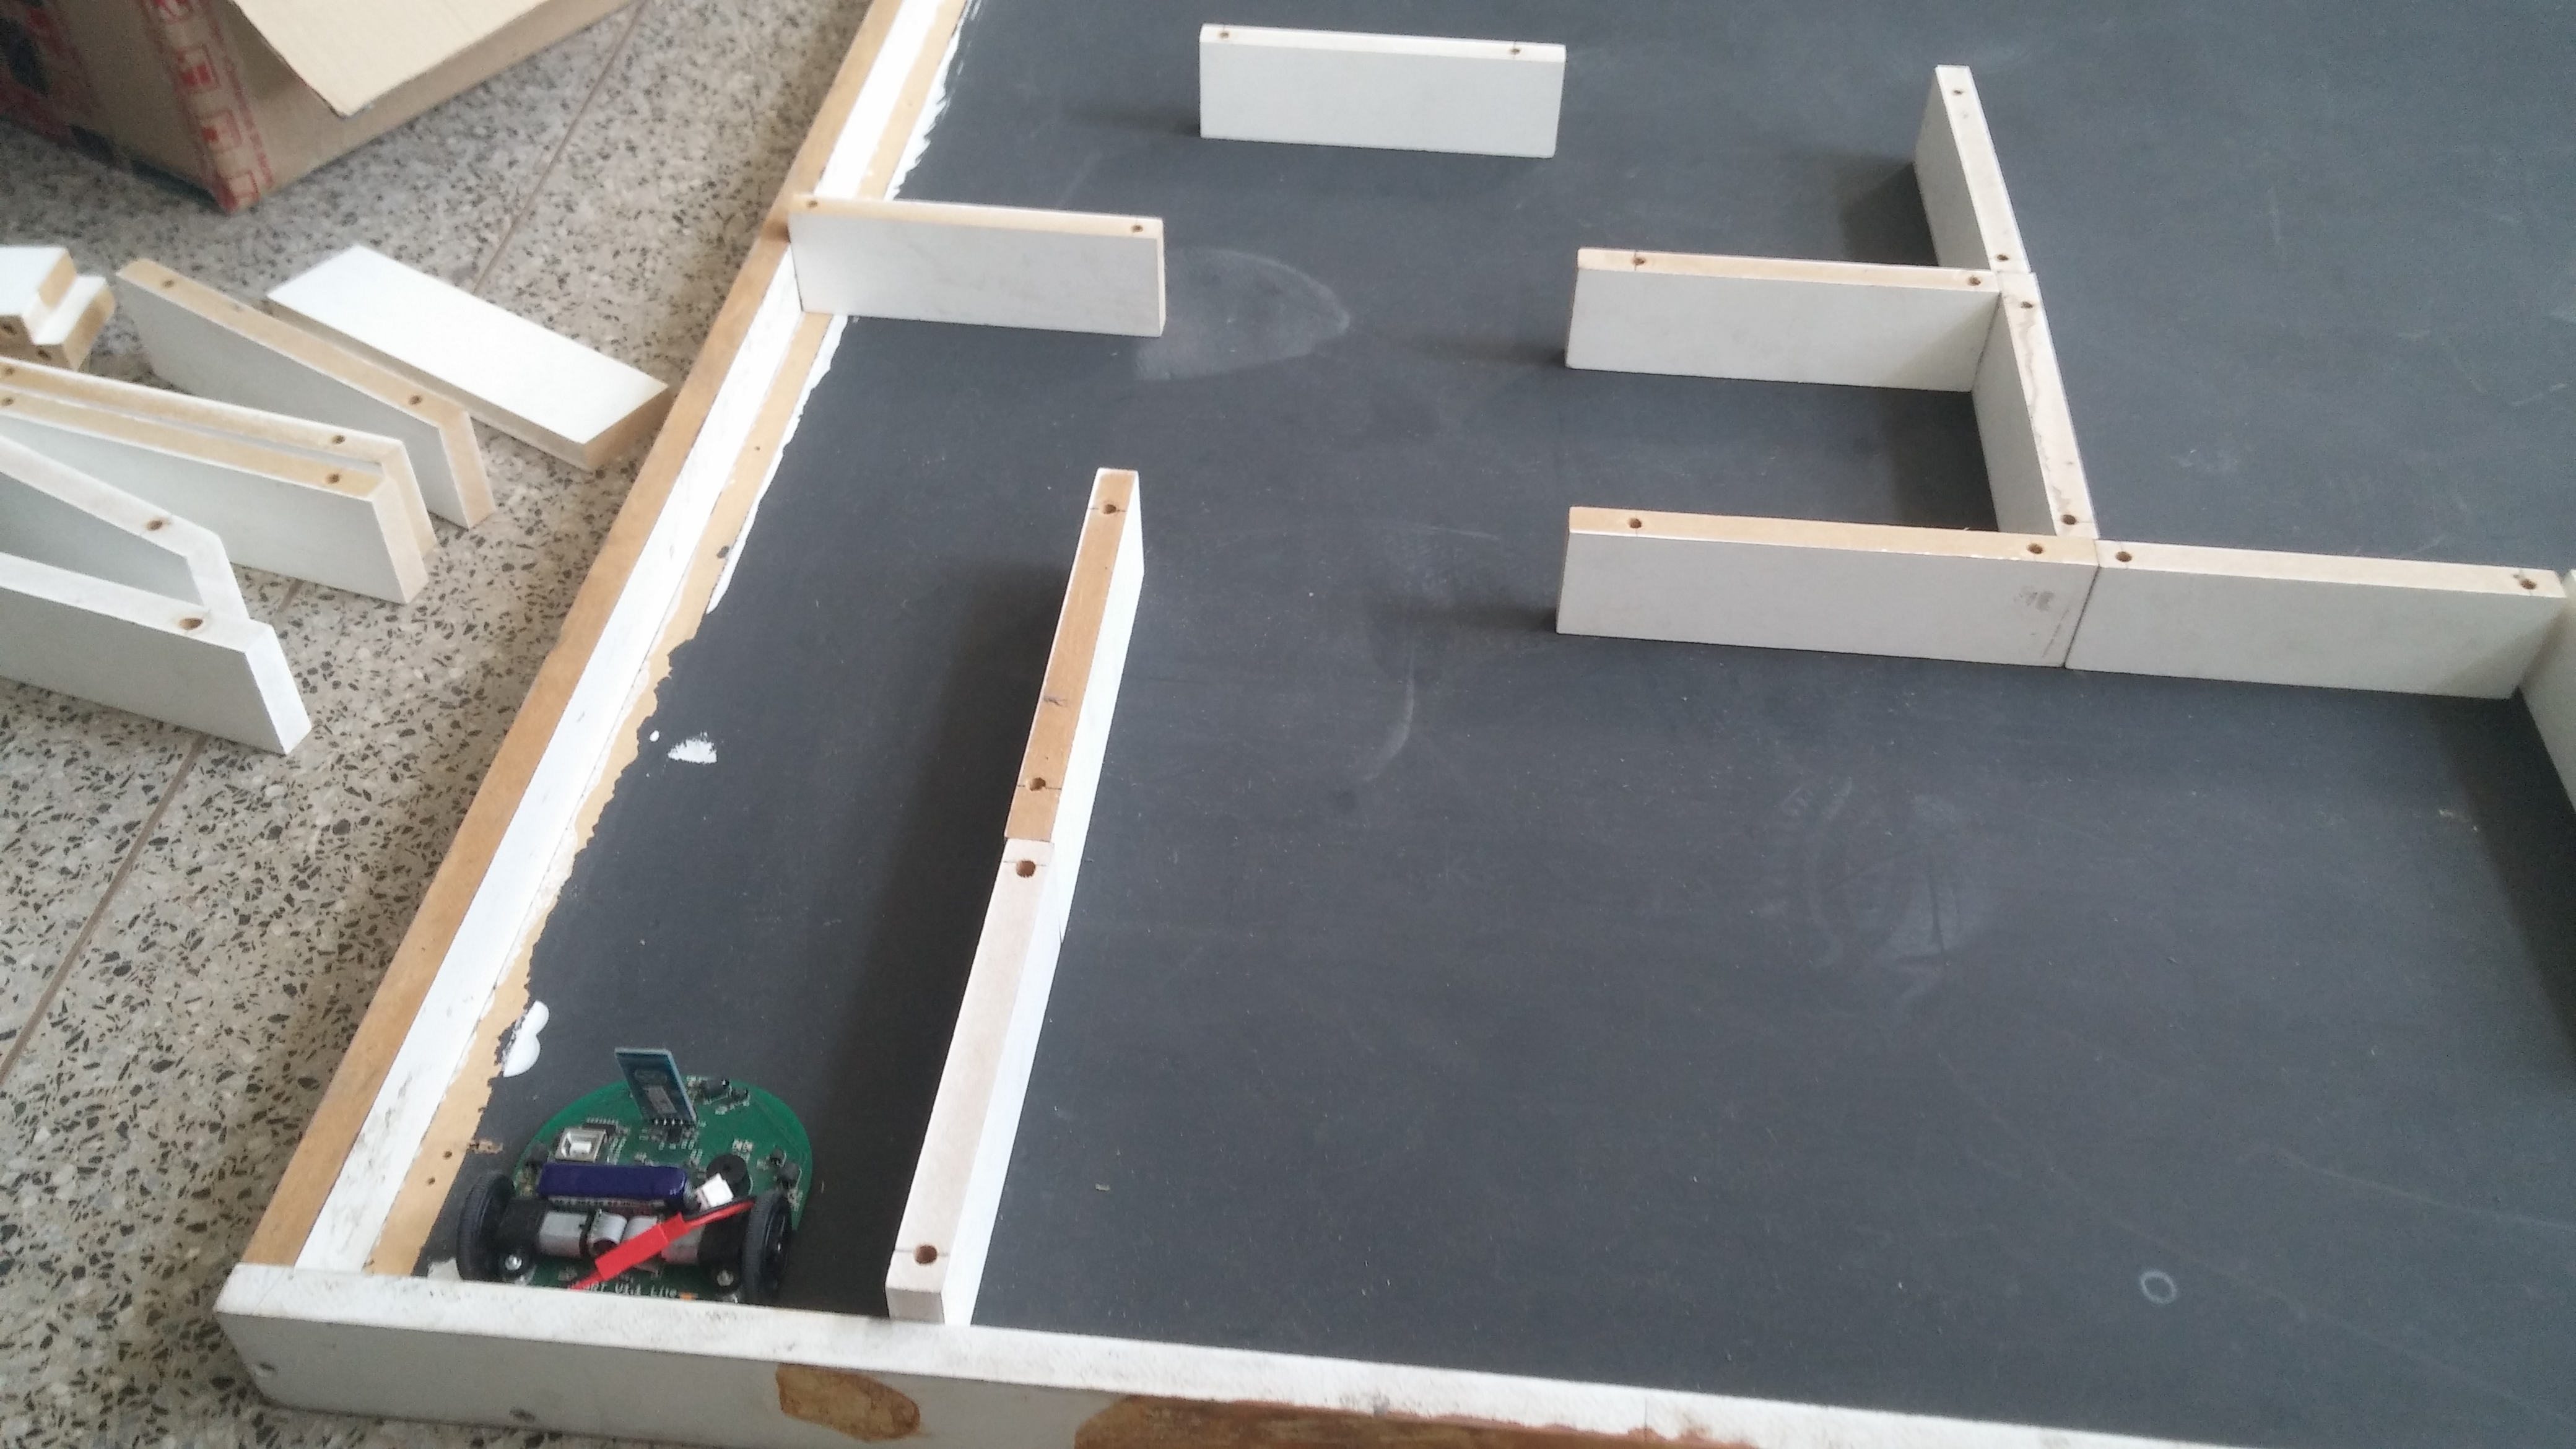
\includegraphics[width=1\linewidth]{primeiroteste.jpg}
	\end{center}
	\legend{Fonte: autor (2017)}
\end{figure}


\subsection{Construção e montagem do labirinto}

Para construção das peças e do tablado, foram utilizadas placas de MDF de $15~mm$ de espessura. Na internet encontram-se fácil esquemas e projetos para montagem de labirinto para testes. Na Figura \ref{fig:proj_labirinto} é apresentada uma maneira simples de construir um labirinto de uma forma que as paredes podem ser trocadas, permitindo diversas configurações para testar o Micromouse. 
 
\begin{figure}[!htb]
	\caption{\label{fig:proj_labirinto}Projeto para contrução de labirinto}
	\begin{center}
		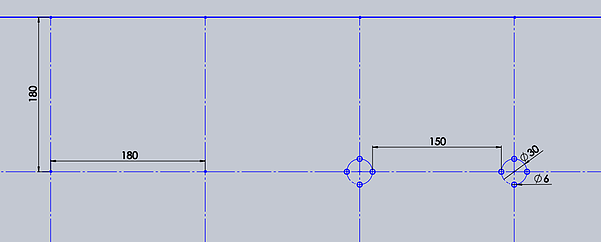
\includegraphics[width=0.9\linewidth]{proj_tablado.png}
	\end{center}
	\legend{Fonte: adaptado de \citeonline{lab:2017}}
\end{figure}

As células de um labirinto oficial medem $180\times180~mm$ (distância entre os centros das paredes). Neste projeto, em cada canto de uma célula (exceto nos limites do labirinto), tem um conjunto de quatro furos de $6~mm$ de diâmetro circunscritos em um círculo com $30~mm$ de diâmetro, conforme mostra a Figura \ref{fig:proj_labirinto}.

\begin{figure}[!htb]
	\caption{\label{fig:medidas_parede}Medidas de corte para as peças}
	\begin{center}
		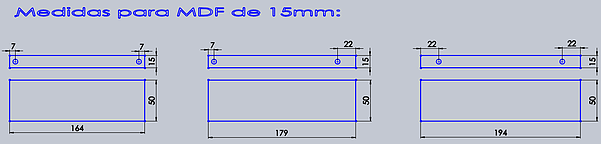
\includegraphics[width=0.9\linewidth]{medidas_parede.png}
	\end{center}
	\legend{Fonte: adaptado de \citeonline{lab:2017}}
\end{figure}

 Neste projeto, são três peças diferentes, conforme pode se observar na Figura \ref{fig:medidas_parede}. Isto possibilita montar qualquer configuração de labirinto. Os furos nestas peças servem para colar cavilhas de madeira (acessório para montagem de móveis) que serão encaixadas nos furos do piso.
As paredes do labirinto foram feitas de MDF com as duas faces pintadas de branco, e o piso, pintado de preto fosco.

\subsection{Testes com labirinto de 8 x 8 células}

O algoritmo é capaz de descobrir o melhor caminho em labirintos de 8$\times$8 células, desde que os seus limites estejam fechadas, exceto a célula-alvo. Através do \textit{EXCEL}, foi modelado um labirinto para testes e seu desenho pode ser visto na Figura \ref{fig:labteste1}.
\begin{figure}[!htb]
	\caption{\label{fig:labteste1}Labirinto-teste de 8x8 células desenhado no \textit{EXCEL}}
	\begin{center}
		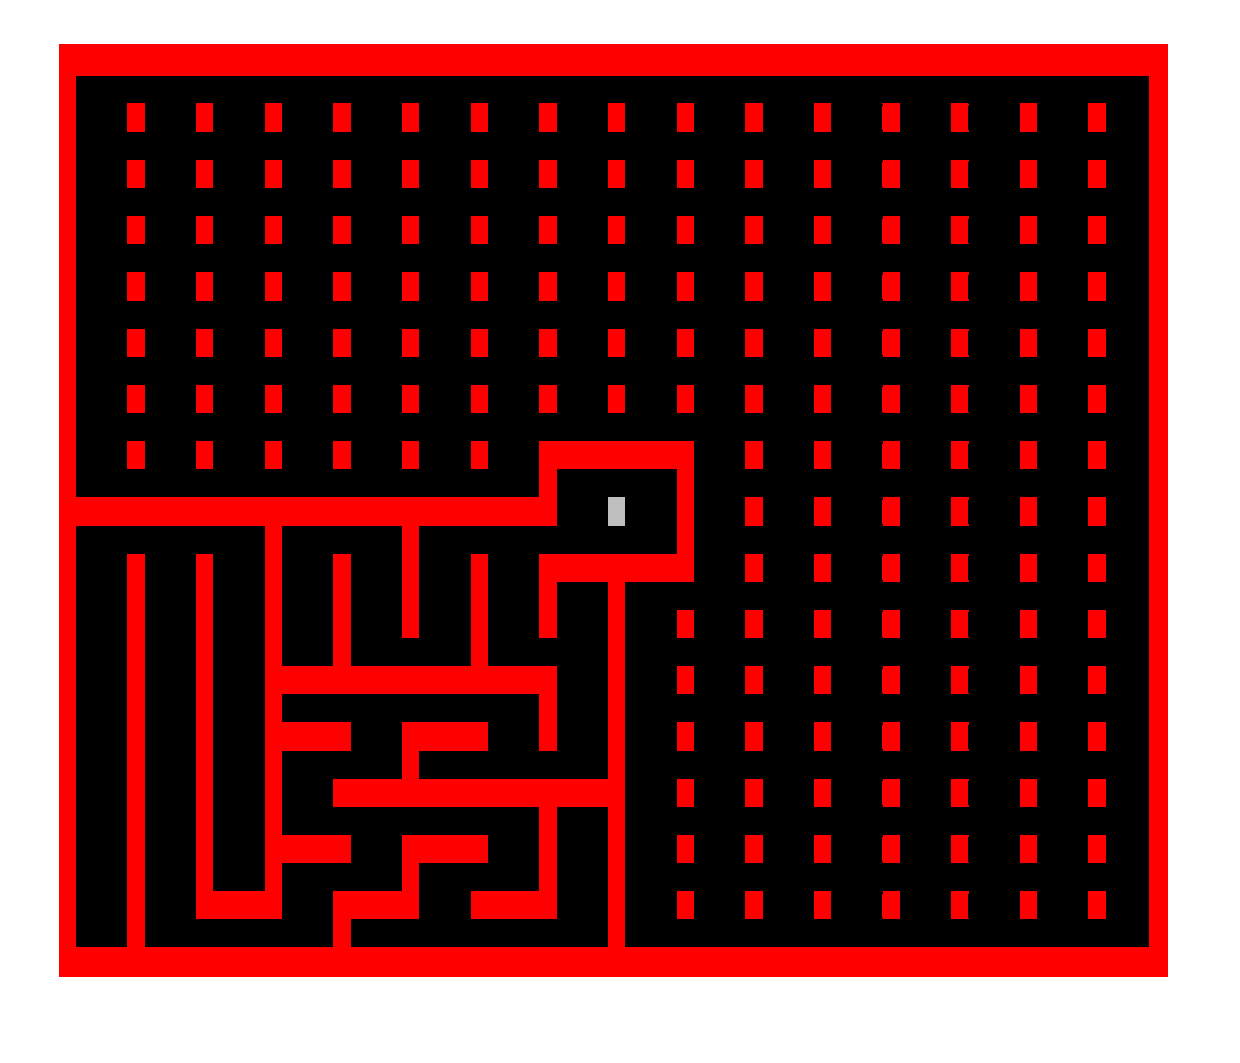
\includegraphics[width=0.55\linewidth]{labirinto_teste.pdf}
	\end{center}
	\legend{Fonte: autor (2017)}
\end{figure}

 As distâncias das células para o melhor caminho podem ser vistas na Figura \ref{fig:labteste2}, onde o percurso otimizado está grifado.
 
\begin{figure}[!htb]
	\caption{\label{fig:labteste2}Labirinto-teste de 8$\times$8 simulado}
	\begin{center}
		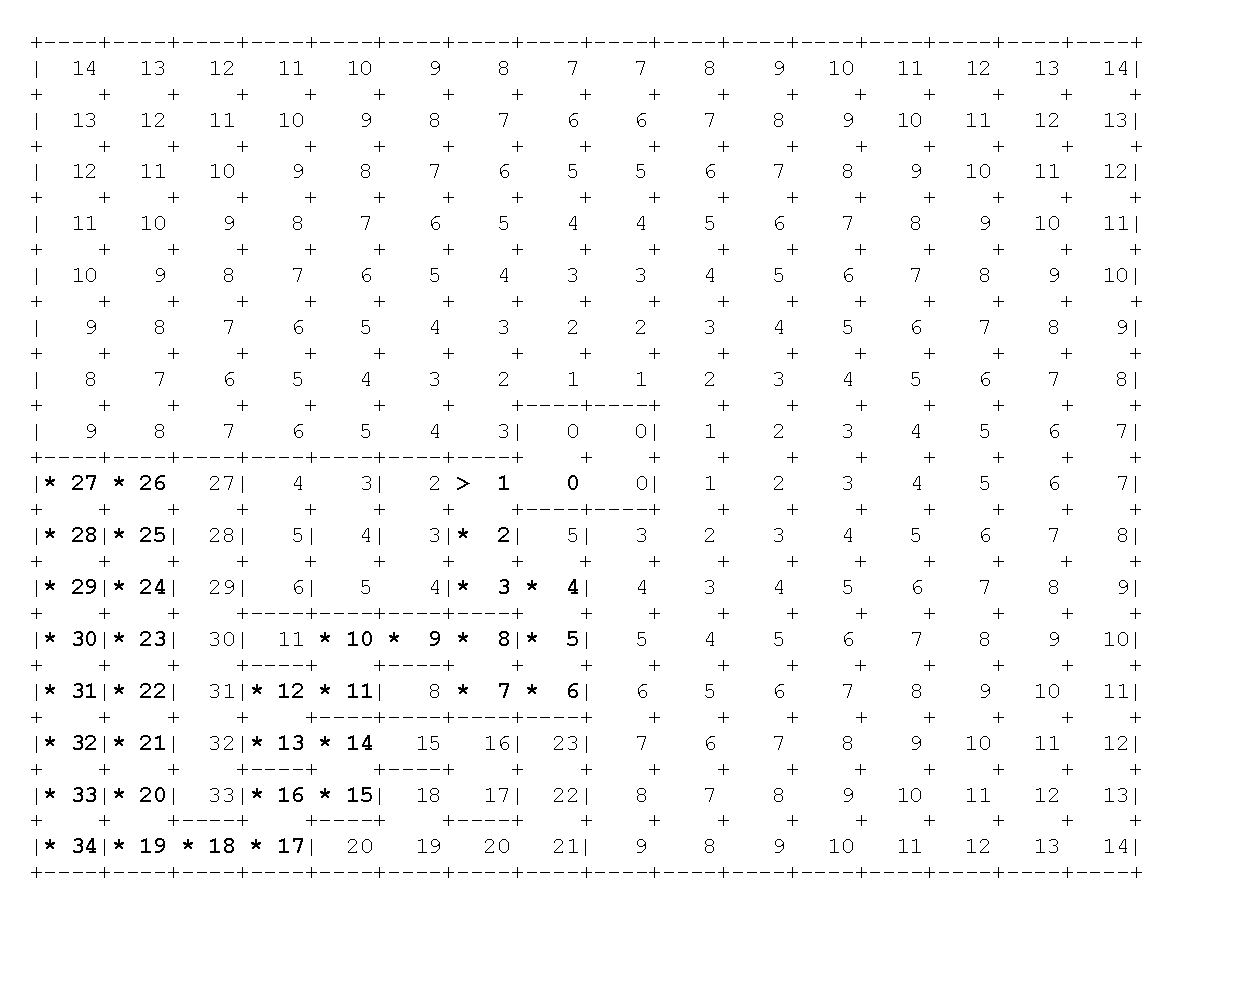
\includegraphics[width=0.6\linewidth]{simulacao_teste.pdf}
	\end{center}
	\legend{Fonte: autor (2017)}
\end{figure}


Então, com as peças disponíveis para montagem, o labirinto-teste foi montado, conforme mostra a Figura \ref{fig:labteste3}.
\begin{figure}[!htb]
	\caption{\label{fig:labteste3}Labirinto montado para testes de 8$\times$8 células}
	\begin{center}
		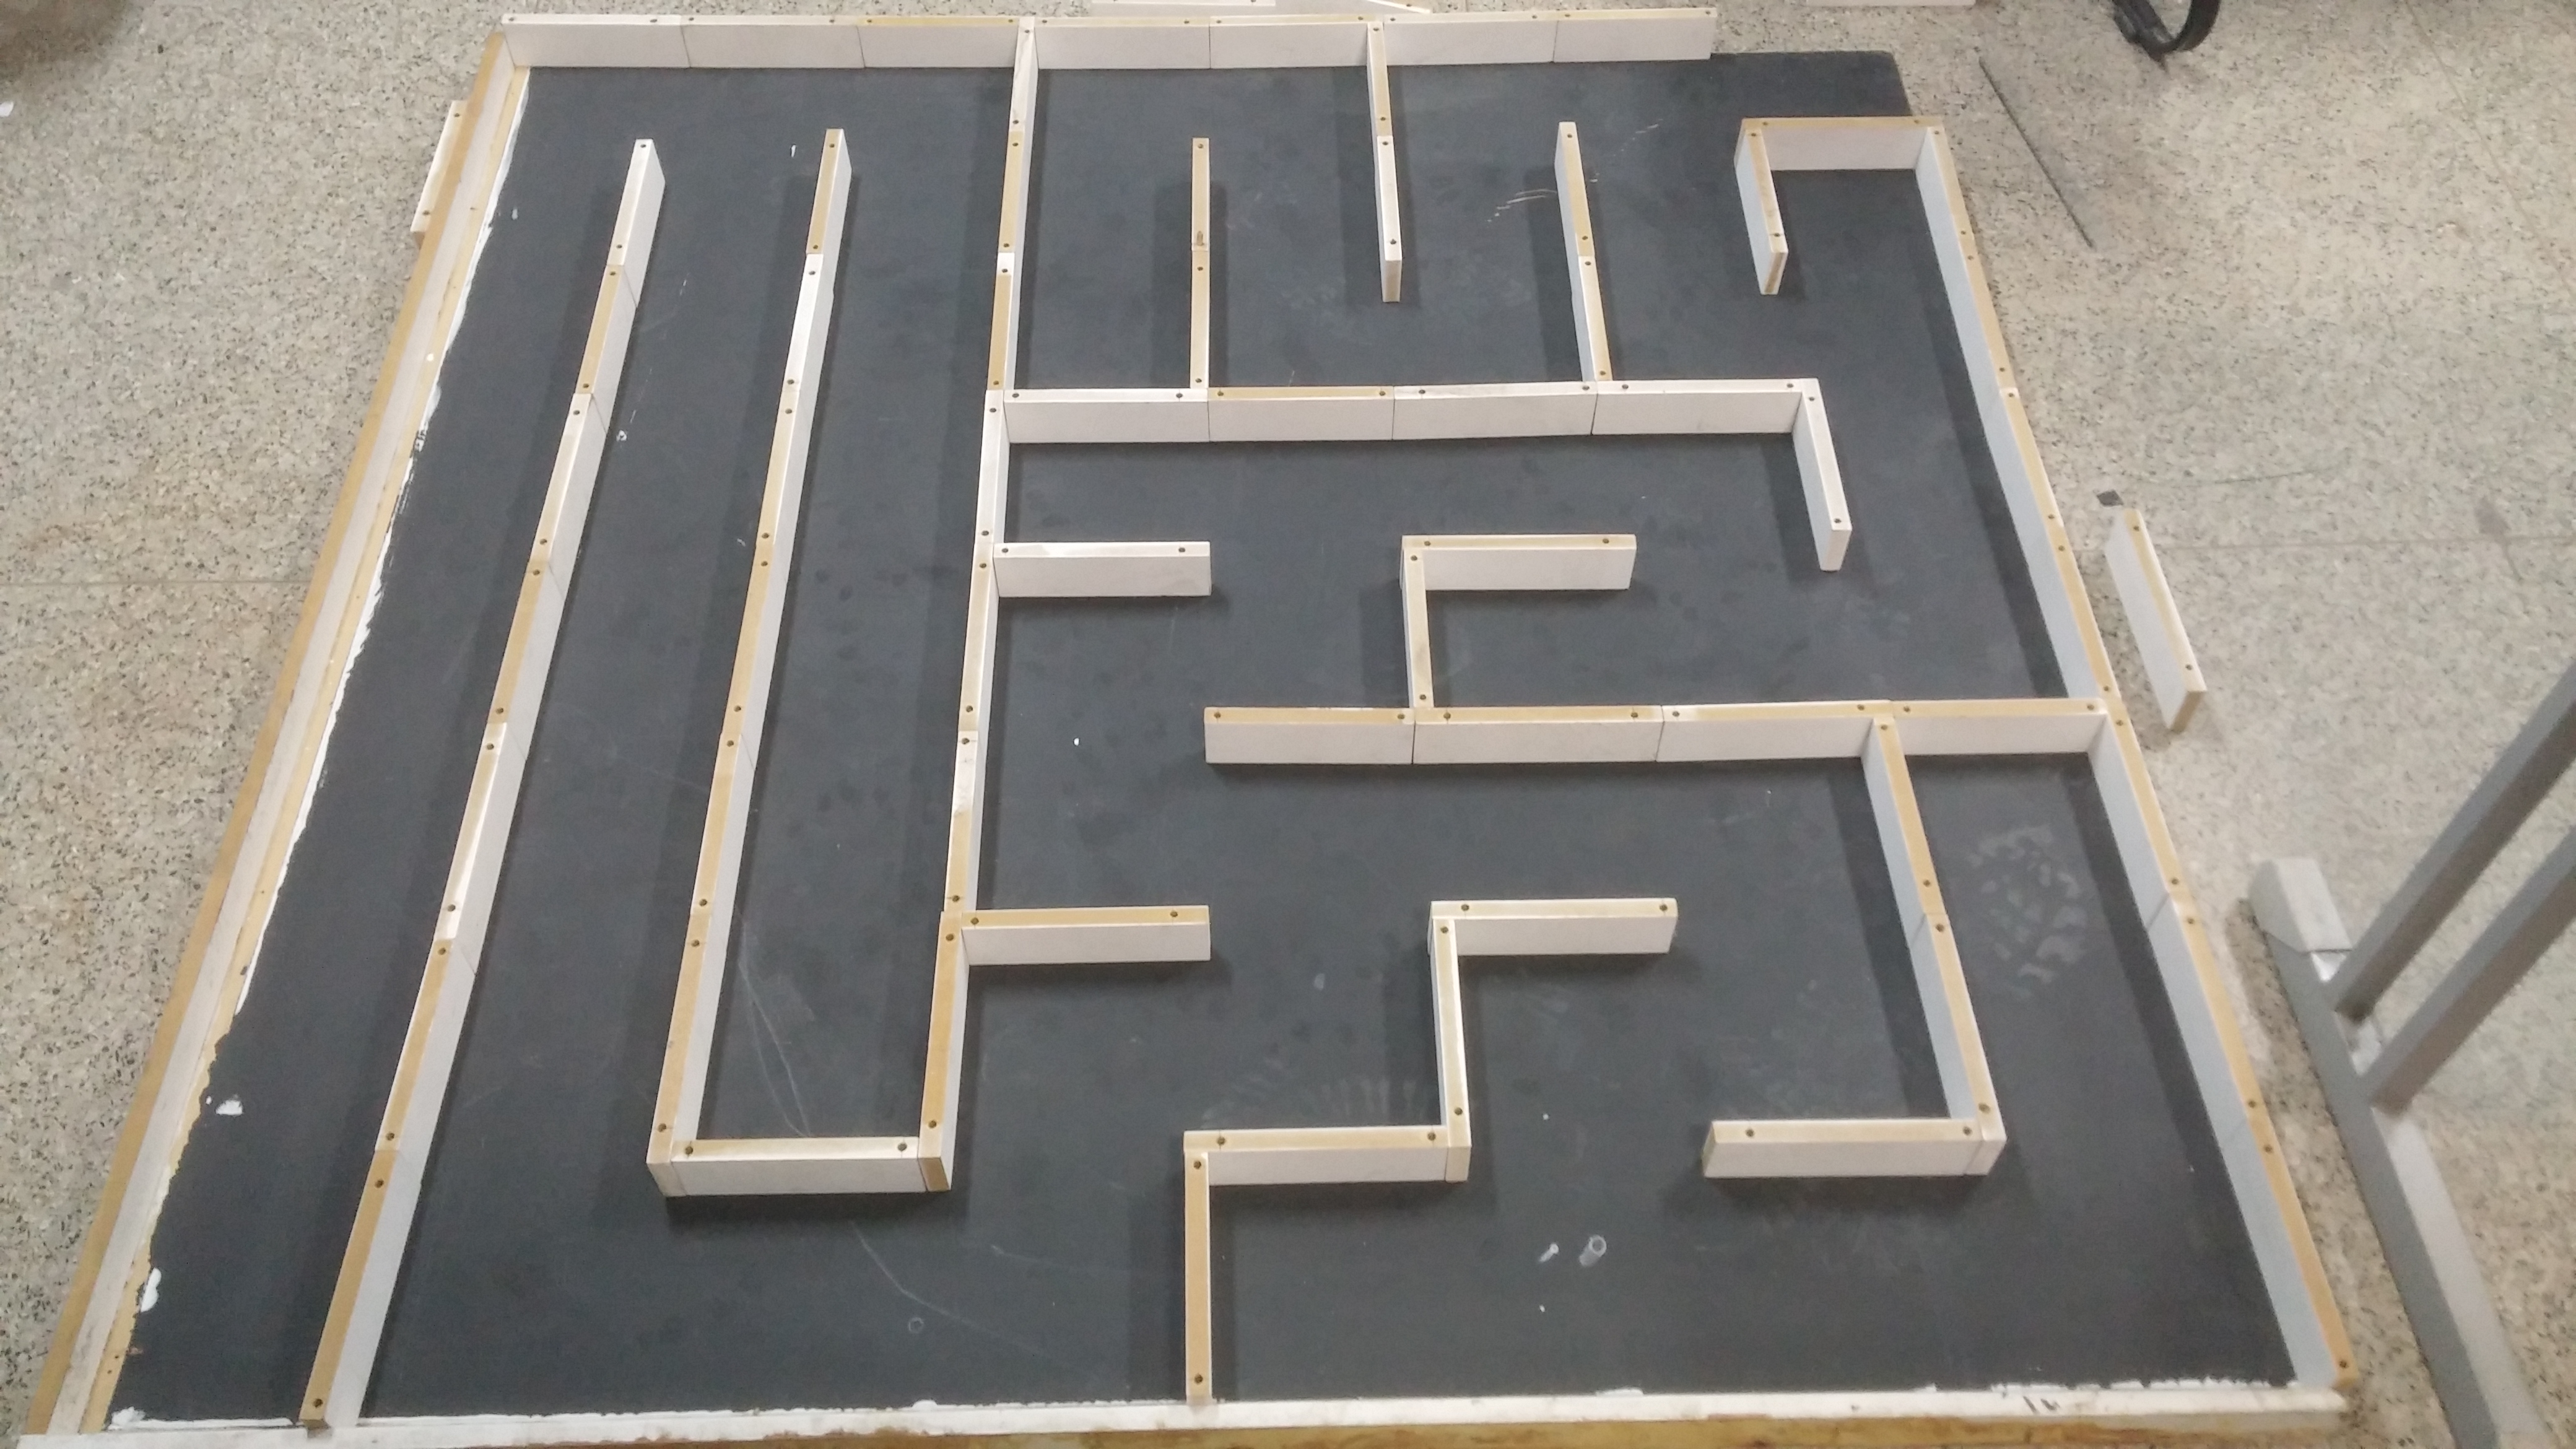
\includegraphics[width=.7\linewidth]{labirinto_8x8.jpg}
	\end{center}
	\legend{Fonte: autor (2017)}
\end{figure}

O sucesso da união das partes propostas construídas e implementadas no robô foi provado pelo êxito do robô em realizar diversas corridas e definir sempre o melhor caminho. A Figura \ref{fig:labteste4} mostra o percurso otimizado do robô para o labirinto-teste montado.
\begin{figure}[!htb]
	\caption{\label{fig:labteste4}Trajetória final do robô sobre o labirinto de 8x8 células}
	\begin{center}
		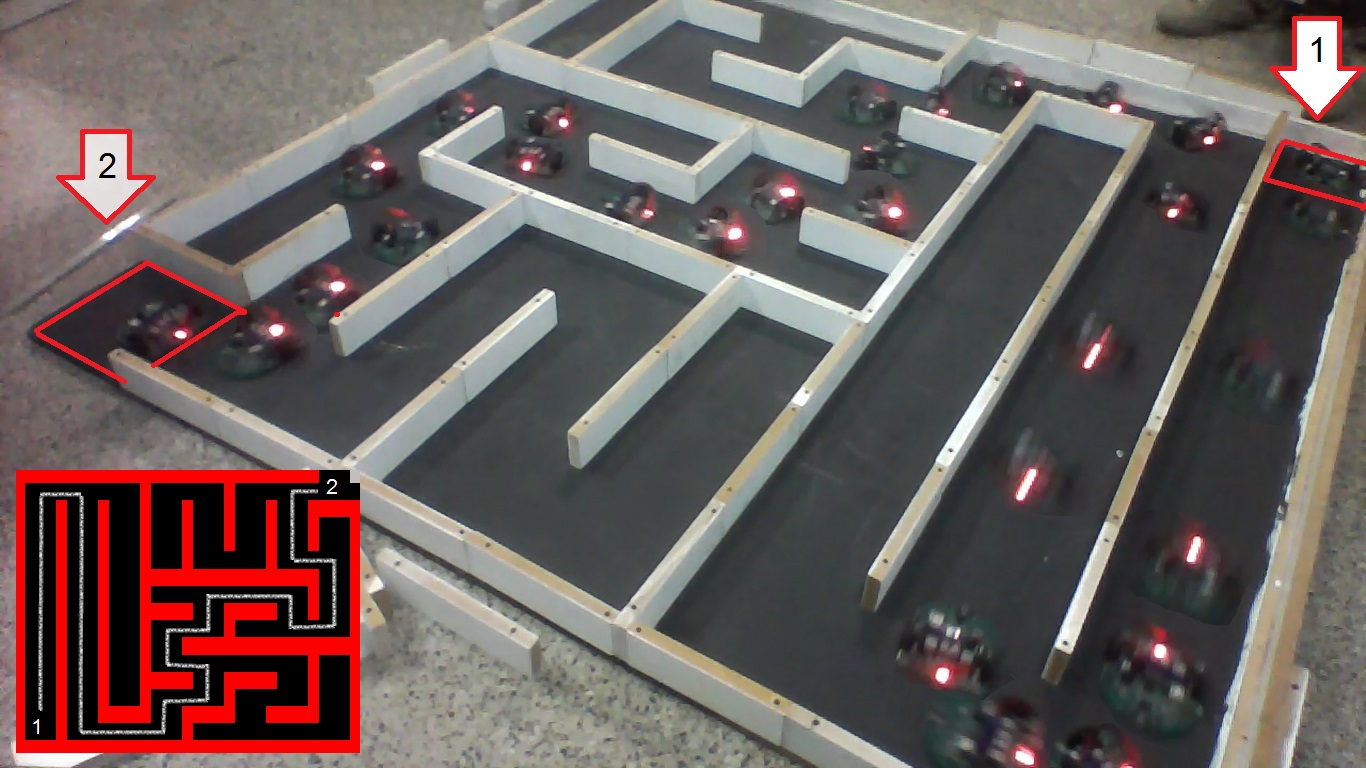
\includegraphics[width=0.8\linewidth]{teste_labirinto.eps}
	\end{center}
	\legend{Fonte: autor (2017)}
\end{figure}

O robô conseguiu resolver o labirinto-teste corretamente e seguiu o mesmo percurso da simulação, tanto na ida como na volta, com velocidade de testes de 30 cm/s em curvas, e 60 cm/s para retas as quais o robô já visitou. 

A correção do erro de posição é feita de forma satisfatória, mantendo o robô paralelamente às paredes, quando elas existem. Os perfis de velocidade, implementados para controlar o movimento, funcionaram como o planejado. O robô realiza as curvas de forma fechada, e lê as informações das paredes antes do início da próxima célula. As acelerações e desalerações ocorreram de forma satisfatória. 


\subsection{Testes com labirinto de 16 x 16 células}


Por fim, o conjunto implementado foi testado e validado num labirinto de 16x16 células. Foram repetidos os procedimentos feitos para o teste do labirinto de 8x8 células.

 
\begin{figure}[!htb]
	\caption{\label{fig:labteste5}Labirinto-teste de 16x16 células desenhado no \textit{EXCEL}}
	\begin{center}
		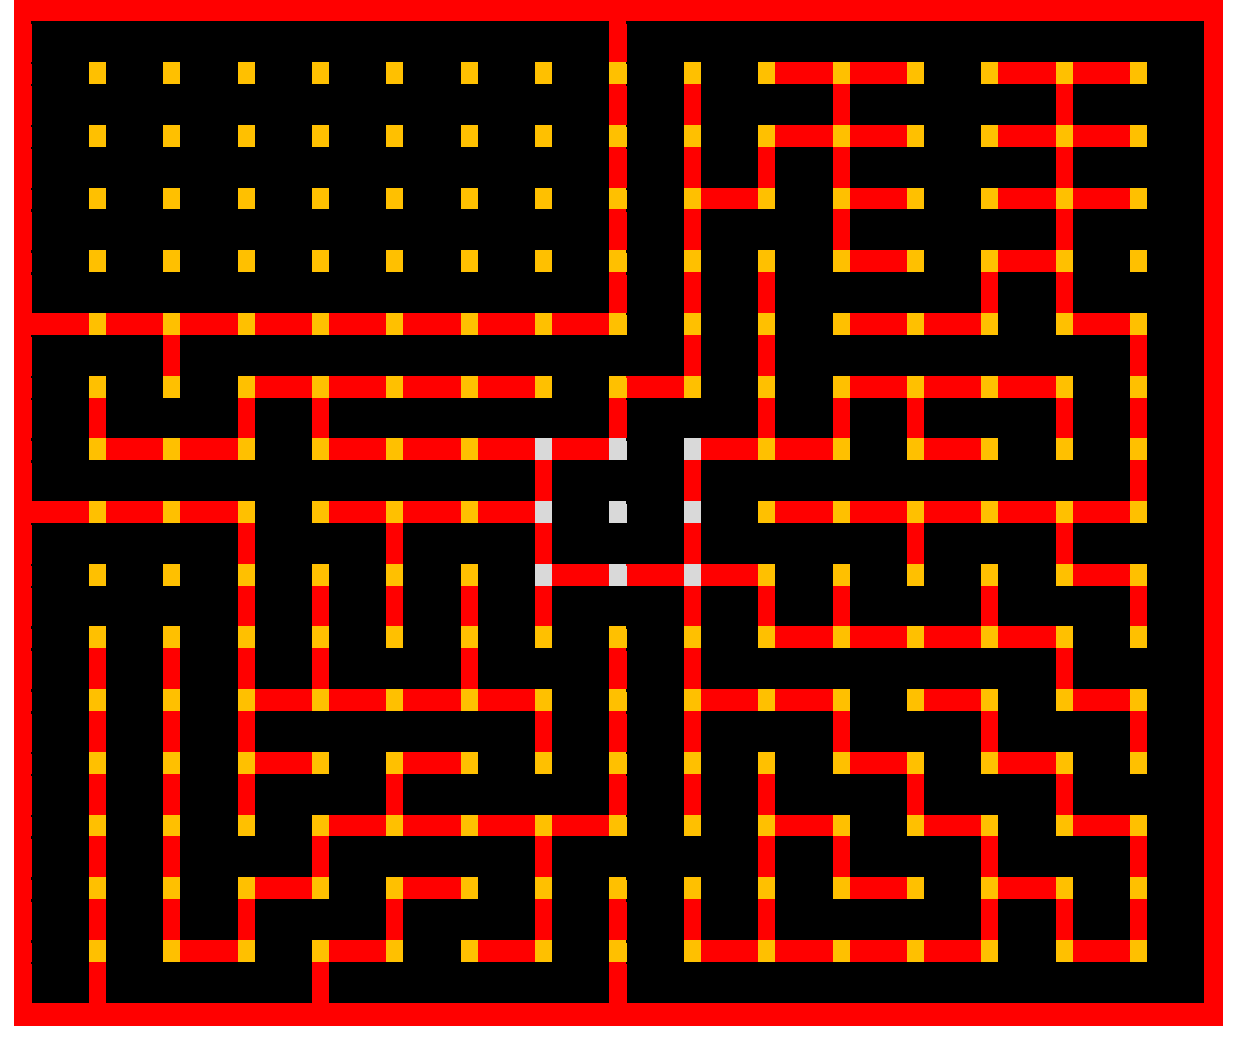
\includegraphics[width=0.7\linewidth]{labirinto_desenhado_16x16_2.pdf}
	\end{center}
	\legend{Fonte: autor (2017)}
\end{figure}

Novamente, através do \emph{EXCEL}, um labirinto foi desenhado de tal forma que as paredes não sejam totalmente conexas. Desta forma, somente os algoritmos inteligentes baseados na Teoria dos Grafos têm capacidade de resolvê-lo. Também, para validação do robô em \emph{malha aberta}, algumas paredes foram retiradas. A Figura \ref{fig:labteste5} mostra o \emph{design} do labirinto proposto.


Para o labirinto-teste de Figura \ref{fig:labteste5}, foram realizadas estatísticas para comparação de desempenho dos algoritmos. A Tabela \ref{tab:estatistica2} mostra em detalhes. 

% algoritmo no maze Downloads

\begin{table}[!htb]
	\centering
	\caption{\label{tab:estatistica2}Desempenho dos algoritmos no labirinto proposto}
\begin{tabular}{c|cc}
 \textbf{Estatíticas} & \textbf{Algoritmo proposto}  & \textbf{\emph{Micro Mouse}} \\ 
\hline 
\textbf{Únicas células atrav.} & 176 & 177 \\ 
\hline 
\textbf{Cél. p/ chegar ao centro (1$^a$ vez)} & 149 & 150\\ 
\hline 
\textbf{Curvas (na primeira corrida)} & 72 & 72\\ 
\hline 
\textbf{Células visit. na melhor corrida} & 68 &  68\\ 
\hline 
\textbf{Curvas (melhor caminho)} & 22 & 22 \\ 
\hline 
\textbf{Cél. atrav. p/ comp. a melhor corrida} & 441 & 578 \\ 
\hline 
\textbf{Curvas (p/ completar a melhor corrida)} & 192 & 228 \\ 
\end{tabular} 
	
	\legend{Fonte: autor (2017)}
\end{table}

O percurso otimizado do Micromouse, para solucionar o labirinto montado, pode ser observado através da Figura \ref{fig:labteste16x16}.

\begin{figure}[!htb]
	\caption{\label{fig:labteste16x16}Trajetória final do robô sobre o labirinto-teste real de 16x16 células}
	\begin{center}
		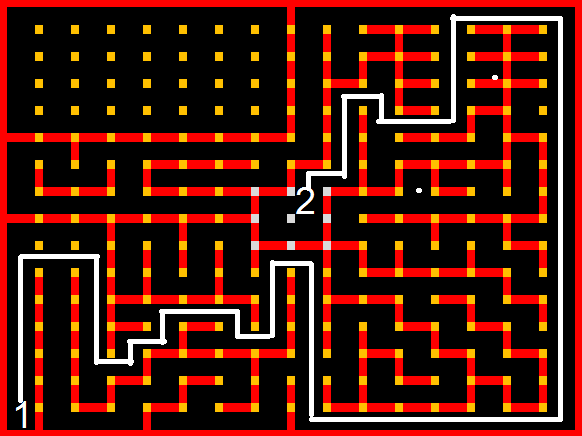
\includegraphics[width=1\linewidth]{teste_labirinto_16x16.eps}
	\end{center}
	\legend{Fonte: autor (2017)}
\end{figure}


Utilizando o \textit{FALCON C++ IDE} para simulação do percurso do robô, os percursos otimizados para o caminho de ida e de volta foram os mesmos do percursos formados pelo robô no labirinto-teste. Os resultados da simulação podem ser vistos na Figura \ref{fig:labteste6}. O menor caminho está marcado com asterisco.

\begin{figure}[!htb]
	\caption{\label{fig:labteste6}Simulação do percurso do robô no labirinto-teste proposto de 16x16 células}
	\begin{center}
		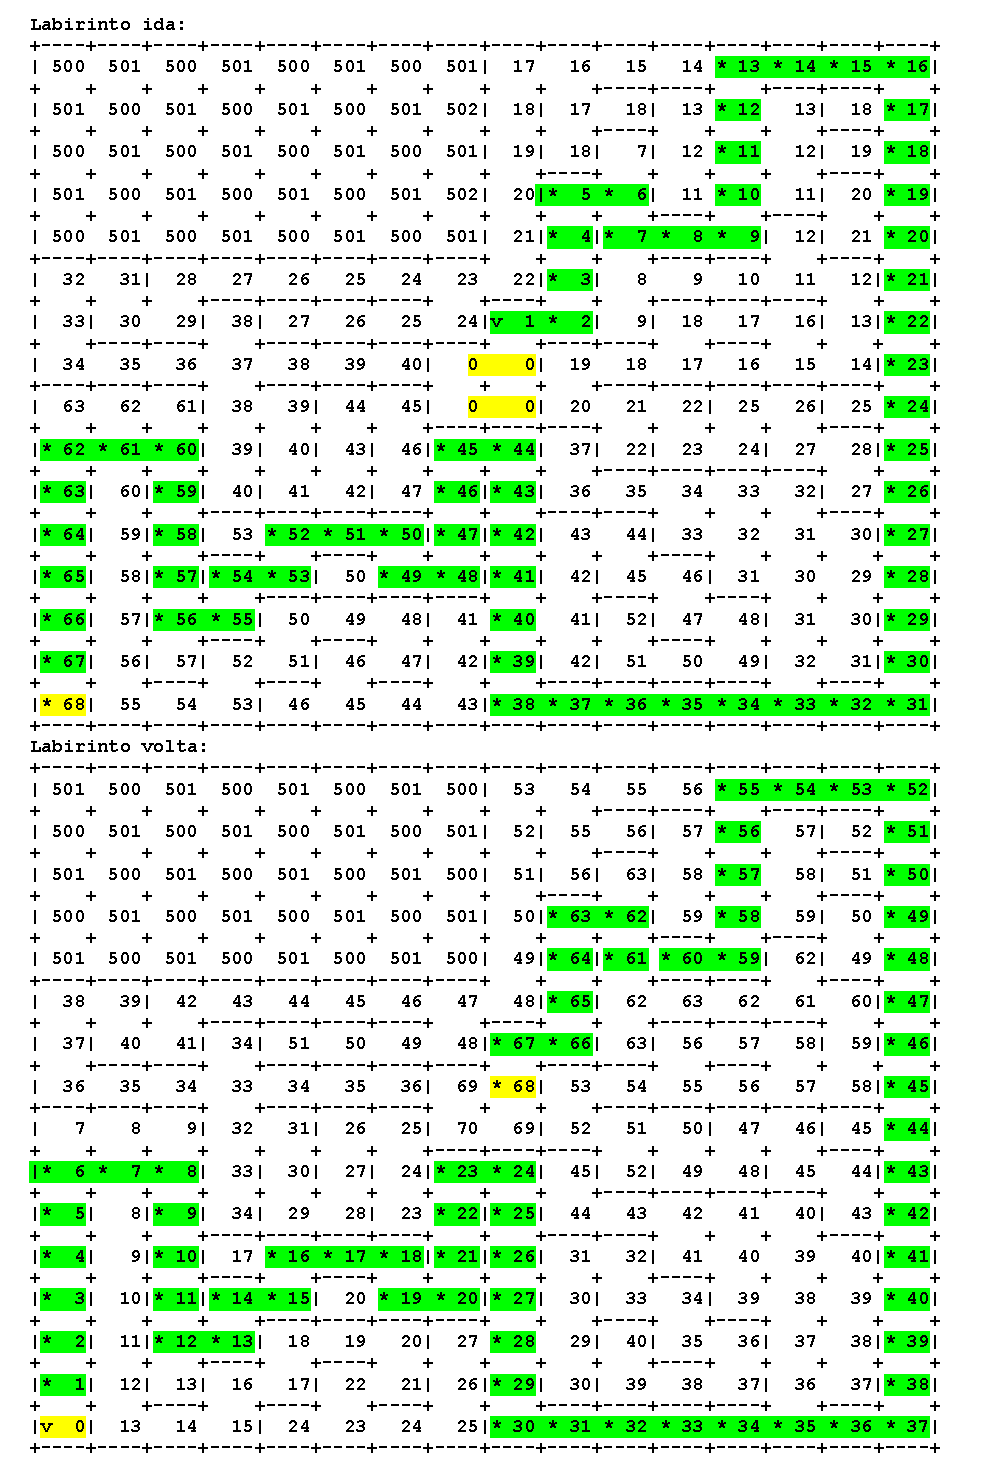
\includegraphics[width=0.7\linewidth]{simulacao_falcon2.pdf}
	\end{center}
	\legend{Fonte: autor (2017)}
\end{figure}



Portanto, no labirinto-teste, o algoritmo proposto já apresenta desempenho superior ao do \emph{Micro Mouse Simulator}. O número de células atravessadas e o número de curvas, para completar a melhor corrida, são inferiores. Isto demonstra que o algoritmo pode apresentar desempenho até superior, a depender do labirinto. E a quantidade de células atravessadas, no percurso de melhor corrida, sempre será igual em ambos os algoritmos implementados.

Para testes em velocidades mais altas, as curvas não são realizadas conforme o esperado. As referências, para tais velocidades, não são seguidas corretamente, visto que, para maiores velocidades tangenciais, são requeridas, também, maiores velocidades angulares para mesmo raio de curva, e, portanto, há um erro em entradas do tipo rampa. O controle clássico implementado somente é adequado para velocidades baixas.